\documentclass{article}
\usepackage{iclr2027_conference,times}
\input{math_commands.tex}
\usepackage{url}
\usepackage{booktabs}
\usepackage{multirow}
\usepackage{amsmath}
\usepackage{amssymb}
\usepackage{graphicx}
\usepackage{float}
\usepackage{algorithm}
\usepackage{algpseudocode}
\usepackage{placeins}
\usepackage{xspace}
\usepackage{hyperref}
\urlstyle{rm}

\title{RISE: Recovery-Informed Scaling via Events for Tool-Using LLMs}

\author{Anonymous Authors}

\newcommand{\method}{RISE\xspace}
\newcommand{\rds}{RDS}
\newcommand{\frd}{FRD}
\newcommand{\api}[1]{\textnormal{#1}}

\hypersetup{hidelinks}
\begin{document}
\maketitle

\begin{abstract}
Stateful LLM tool calling can fail even after the model recognizes an anomaly and enters recovery: it may choose the wrong recovery target, action, arguments, order, verification procedure, or stopping decision. We distinguish Failed Recovery Decisions (FRD), adjudicated from an evidence-complete recovery episode and its adverse outcome, from Recovery-risk Disagreement Signals (RDS), public evidence available during execution without final evaluator labels. We introduce RISE (Recovery-Informed Scaling via Events), a test-time scaling framework that uses RDS to focus fresh complete rollouts, retains an accepted incumbent, and updates source-constrained bilateral event guidance after candidate comparison. Across StateBench, AppWorld, OccuBench, and DeepPlanning Travel, RISE improves aggregate metrics over Vanilla and Best-of-4 for three LLMs.
\end{abstract}

\section{Introduction}

LLM tool calls can mutate an external environment, so later calls must remain consistent with earlier effects. A failed update, an unexpected empty result, or a stale object identifier can turn a locally plausible continuation into an invalid task state. Reliable tool calling therefore requires grounding targets and arguments, respecting preconditions, preserving mutation order, and verifying consequential state changes.

\textbf{A successful recovery action does not necessarily restore task progress.} Figure~\ref{fig:frd-phenomenon} shows a real AppWorld case: the LLM must inspect reminder drafts and delete only those associated with replied-to job applications. Baseline A requests the drafts without an \api{access\_token} at A08 and receives a 401 error. It obtains a token by logging in at A36, but omits the token again when retrying at A50, repeating the authentication failure. This example illustrates one form of FRD: the retry fails to apply a prerequisite established during recovery. Assessing recovery therefore requires examining the recovery decision and the resulting dependent behavior.

This case is one instance of a Failed Recovery Decision (FRD): entering recovery does not ensure that the LLM chooses the correct target, action, arguments, ordering, verification procedure, or stopping decision. More generally, FRD can arise at the first recovery attempt, across dependent tools, or after a superficially successful action that leaves the recovery state degraded. The error message, retry arguments, and repeated failure expose Recovery-risk Disagreement Signals (RDS). FRD is adjudicated retrospectively from an evidence-complete recovery episode and its adverse outcome, whereas RDS is extracted from public evidence available during execution without final evaluator labels. Because a local recovery failure does not determine the final task outcome, we ask: \emph{given additional complete executions, how should public recovery evidence focus the next attempt and how should candidate comparison update later guidance?}

\begin{figure}[!htb]
\centering
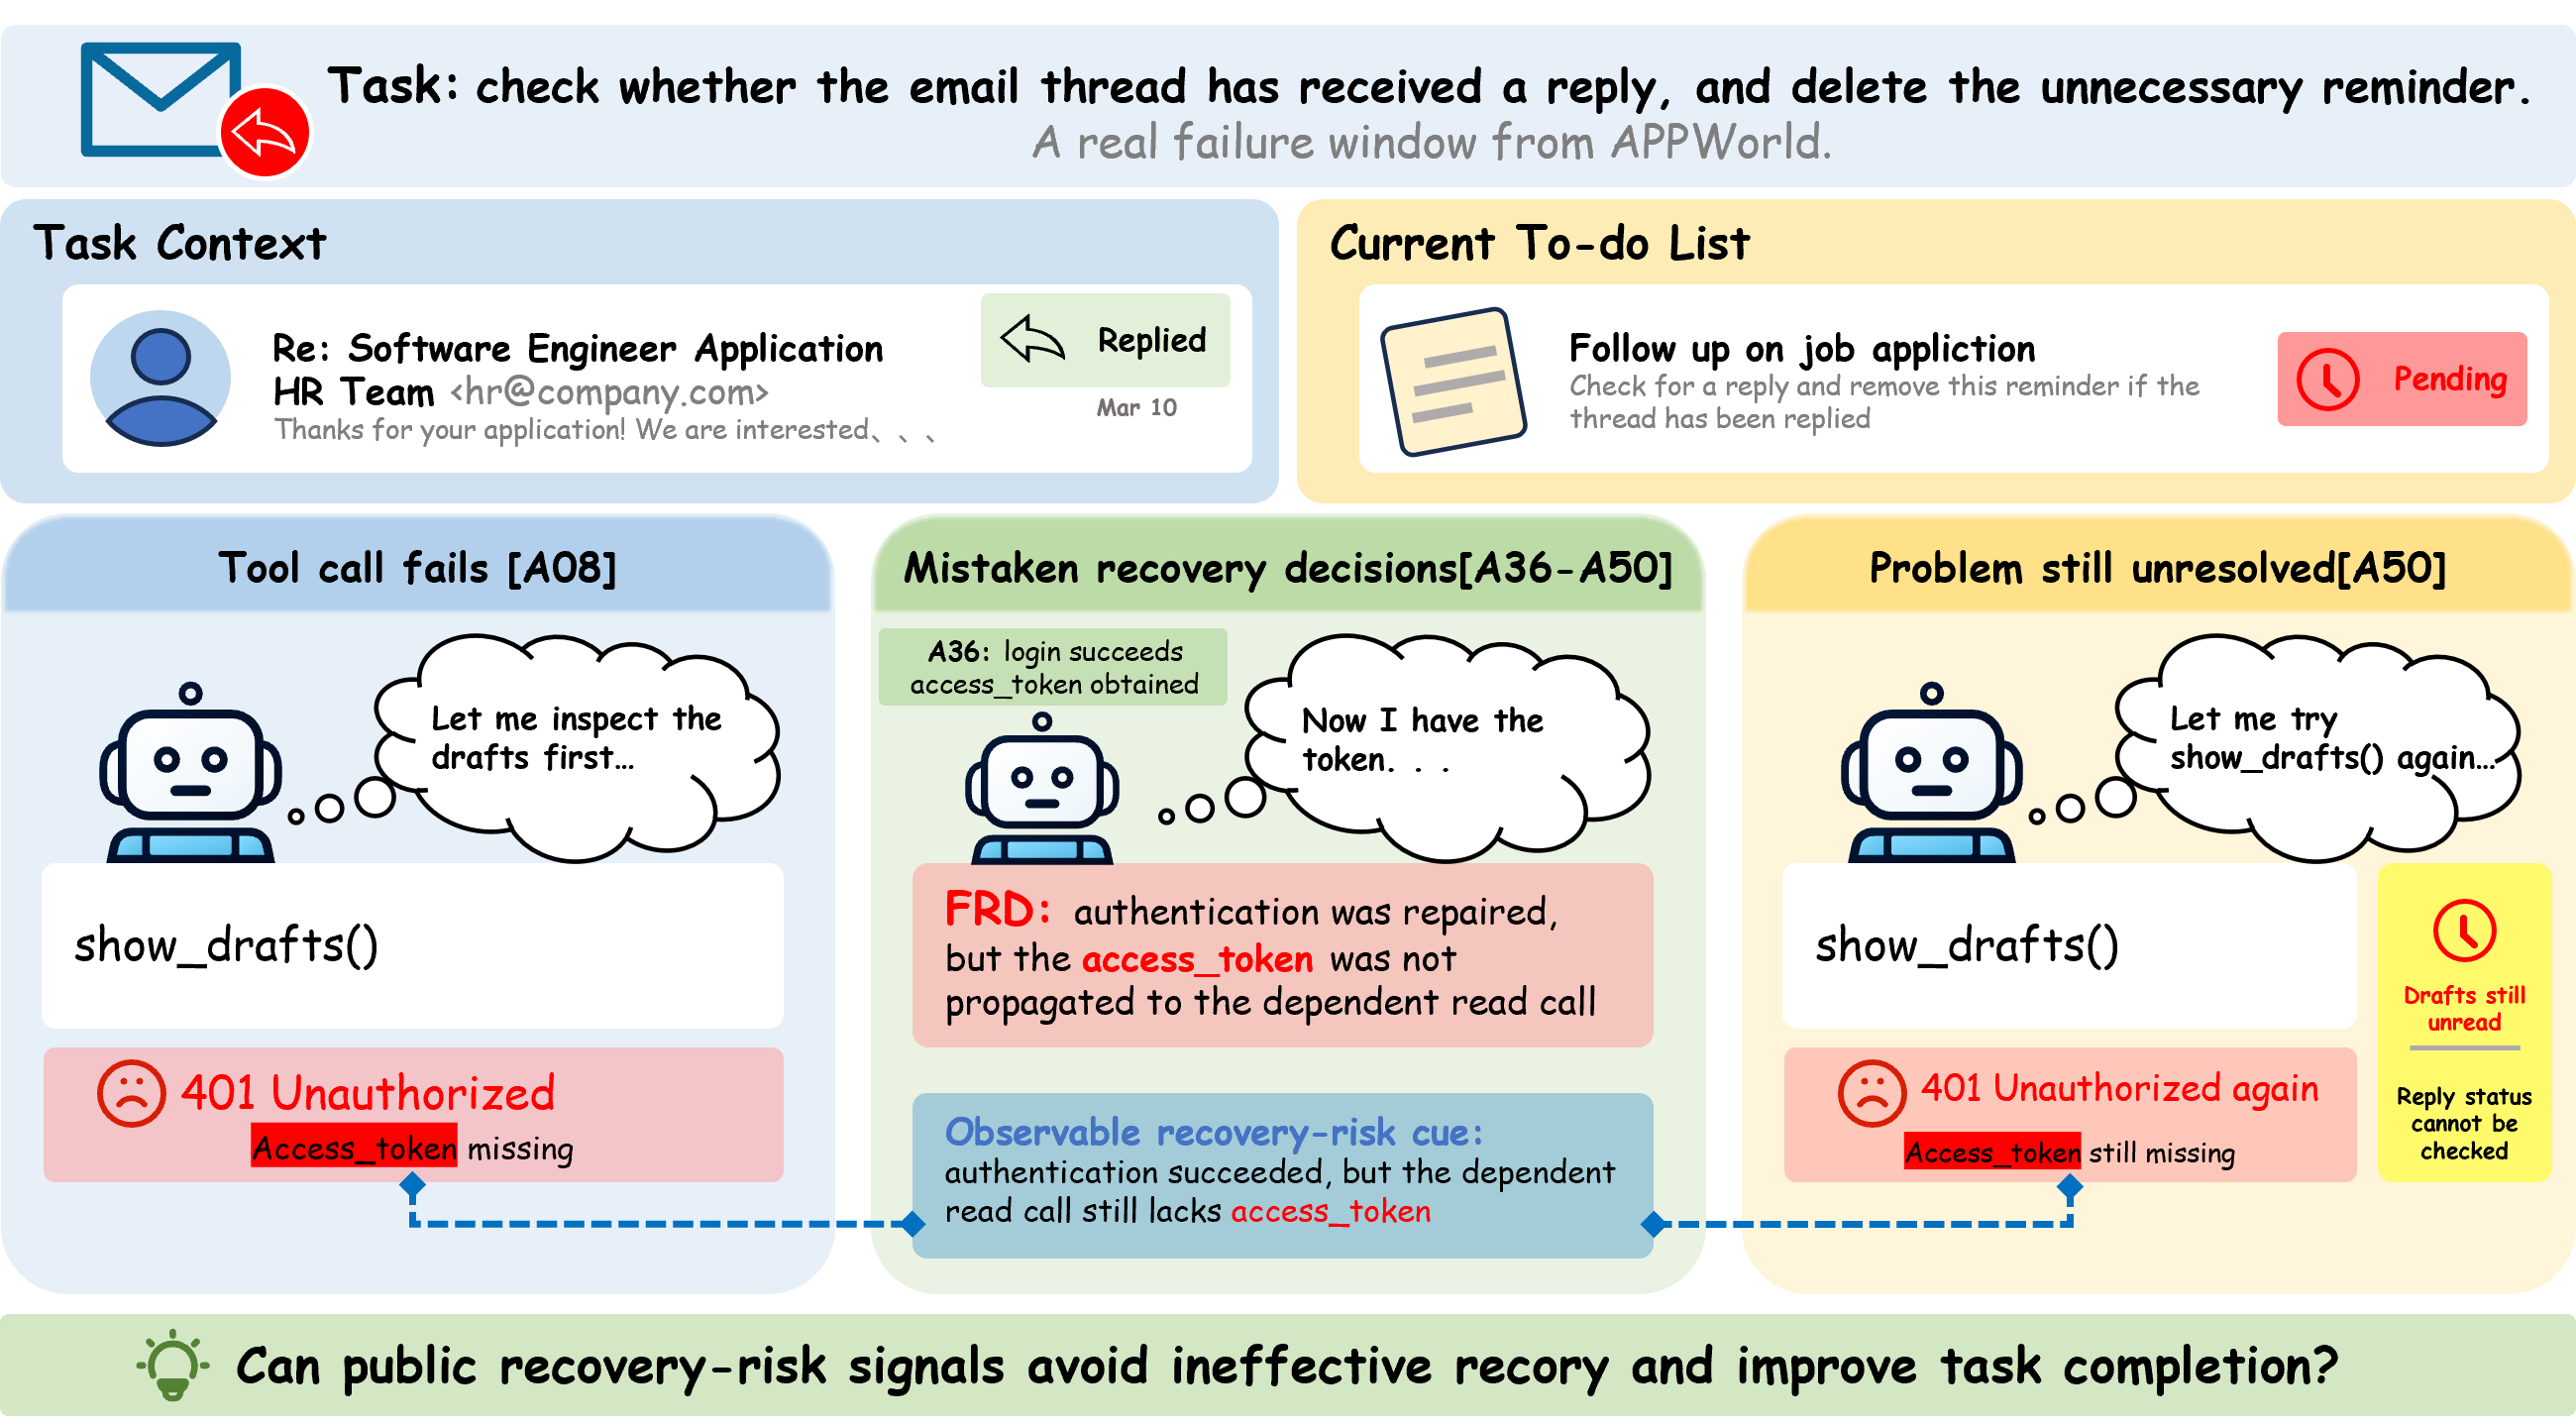
\includegraphics[width=0.85\linewidth]{figures/frd_phenomenon.png}
\caption{Baseline A logs in at A36 but omits \api{access\_token} at A50, repeating the authentication error at A08. Obtaining a token alone does not complete recovery. Intermediate turns are omitted.}
\label{fig:frd-phenomenon}
\end{figure}

Prior work has improved tool-use data, trajectory representations, and inference-time selection. ReAct interleaves reasoning, tool calls, and observations \citep{yao2023react}. OAgents studies design choices for tool-using LLM systems, and its test-time-compute study evaluates parallel sampling, sequential revision, verification, and result merging \citep{oagents2025,oppo_tts2025}. Its released four-rollout configuration uses Best-of-$N$ sampling with list-wise verification and result merging, providing a strong Best-of-4 comparison under the same rollout budget. These methods select among completed trajectories. RISE studies how to organize RDS-directed execution, complete-trajectory retention, and bilateral event guidance in one accepted-incumbent search, without accessing hidden state or final evaluator labels.

We propose \method (Recovery-Informed Scaling via Events) to address this organization problem. RDS determines what the next fresh rollout should recheck; complete-candidate comparison determines which trajectory becomes the accepted incumbent; and source-constrained feedback from both candidates determines which structures the next round may preserve, avoid, or revisit. These updates form one recursive search rather than independent controllers. Section~\ref{sec:rise} describes this recovery-aware scaling process.

We compare RISE with Vanilla and Best-of-4 on StateBench, AppWorld, OccuBench, and DeepPlanning Travel. Aggregate metrics improve for all three evaluated LLMs. Our contributions are:
\begin{itemize}
    \item We define FRD as an evidence-complete recovery failure and RDS as publicly observable recovery-risk evidence available without final evaluator labels, and analyze how the two signals relate to task completion under the stated adjudication protocol.
    \item We introduce RISE, which combines RDS-directed fresh complete rollouts, accepted-incumbent search, and source-constrained bilateral event feedback for subsequent LLM tool-calling rounds.
    \item We evaluate RISE against Vanilla and Best-of-4 on four benchmarks, reporting aggregate gains for three LLMs and descriptive recovery analyses on three tool-calling benchmarks.
\end{itemize}

\section{FRD and RDS in LLM Tool Calling}
This section separates the offline recovery label from the online evidence used to guide later LLM tool-calling rollouts. We first define FRD and RDS, then measure their prevalence across benchmarks, and finally examine how FRD-associated trajectories relate to task completion. Unless stated otherwise, the quantitative analyses and plots in this section use DeepSeek-v4.1-Flash.

\subsection{Definitions}
FRD is a harmful recovery decision identified after execution from a complete evidence chain; RDS is public recovery-risk evidence available during execution without final evaluator labels.
Let $\tau=(a_1,o_1,\ldots,a_T,o_T,r)$ be a tool-calling trajectory, with actions $a_t$, public observations $o_t$, and final response $r$. For an audited recovery episode $w\in\mathcal{W}(\tau)$, let $F_w,D_w,I_w,L_w$ indicate a recovery need, a recovery attempt, an incorrect decision, and an adverse recovery outcome attributable to that decision. Recovery attempts include concrete diagnosis or planning. A recovery need may begin with an initial anomaly, user-reported problem, or inconsistent state; it does not require an earlier failed tool call. An adverse outcome includes leaving the target unrecovered, violating a recovery constraint, a tool rejection, or a successful action that still violates a known recovery constraint. We define
\begin{equation}
\mathrm{FRD}(\tau)=\mathbf{1}\!\left[\exists w\in\mathcal{W}(\tau):F_wD_wI_wL_w=1\right].
\end{equation}
We record three outcomes separately: whether an evidence-complete FRD was detected, whether the recovery episode ended as restored, unresolved, or unknown, and whether the benchmark task ultimately passed. A later successful recovery does not erase an earlier FRD, and an FRD does not imply final task failure.
A recovery need may arise from an unmet recovery goal or an inconsistent observation even without an explicit tool error, whereas task failure alone does not establish FRD. The episode must contain a concrete recovery entry or decision and enough evidence to attribute an adverse recovery outcome to that decision. Online, $R_{\tau,j}=g_b(x,\tau_{\leq j})$ collects single-trace RDS evidence from task $x$ and the public trace prefix through action $j$ in benchmark $b$, including failure boundaries, repeated mutations, missing read-back, and explicit API failures. Its online character means that it does not depend on the final evaluator label; in RISE it primarily guides the next fresh complete rollout rather than taking over the current tool call. After a proposal is complete, pairwise comparison can add a separate candidate-disagreement signal for later guidance. Single-trace RDS and candidate disagreement are therefore distinct public signals. RDS is a cue for what should be rechecked, not an FRD label or calibrated success probability.

\subsection{Cross-benchmark prevalence}
We next ask whether these signals recur across LLM tool-use benchmarks. The quantitative analyses and figures in this section use DeepSeek-v4.1-Flash. Figure~\ref{fig:frd-rds-distribution} reports detected FRD and RDS prevalence under the stated adjudication protocol. RDS evidence is observable in all three benchmarks, highest on StateBench and lowest on AppWorld; detected FRD is lower in every benchmark because it additionally requires a complete evidence chain and an attributable adverse outcome, remaining below 10\%. Best-of-4 generally lowers detected FRD and lowers RDS on StateBench and AppWorld, while the change on OccuBench is smaller. Overall, FRD and public recovery-risk evidence recur across all three environments and remain observable after Best-of-4 selection. Their persistence motivates using recovery evidence to guide subsequent rollouts alongside complete-trajectory selection.

\begin{figure}[!htb]
\centering
\begin{minipage}[t]{0.46\linewidth}
\vspace{0pt}
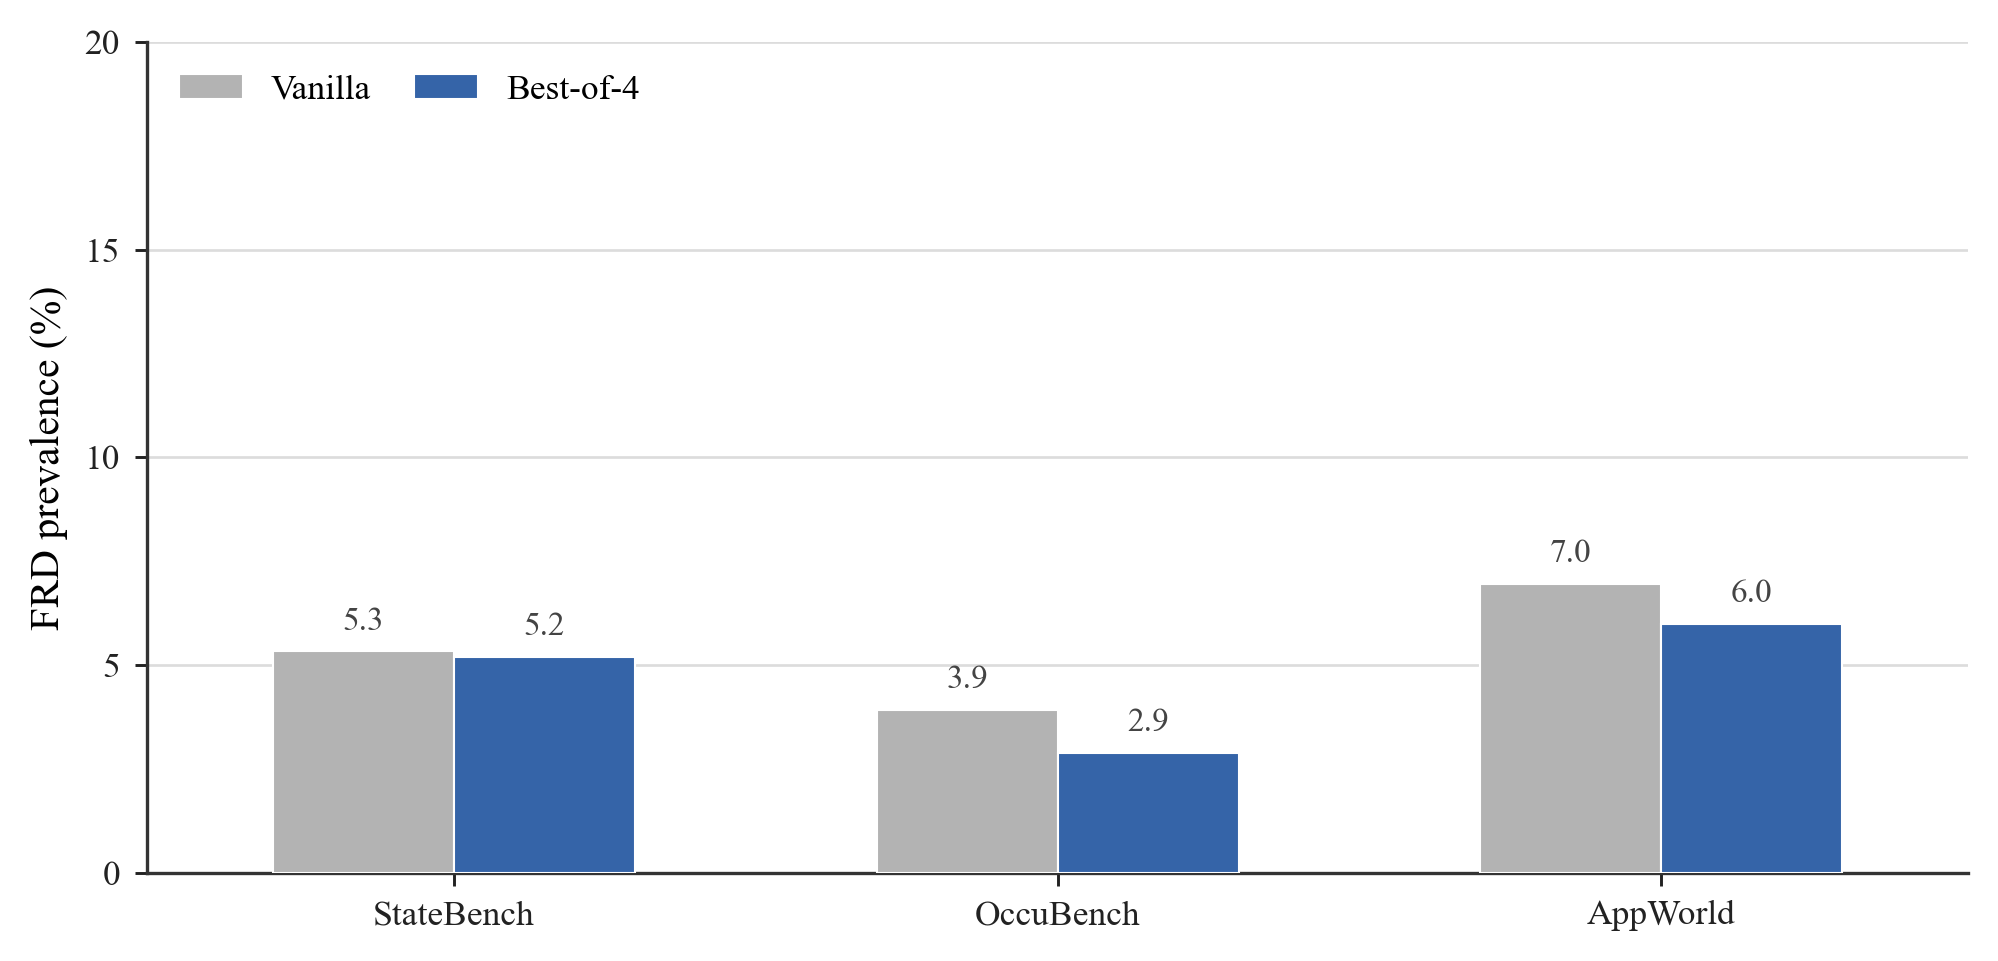
\includegraphics[width=\linewidth]{figures/baseline_frd.png}
\par\vspace{4pt}\raggedright\normalfont\normalsize
(a) FRD prevalence.\par
\end{minipage}\hspace{0.02\linewidth}
\begin{minipage}[t]{0.46\linewidth}
\vspace{0pt}
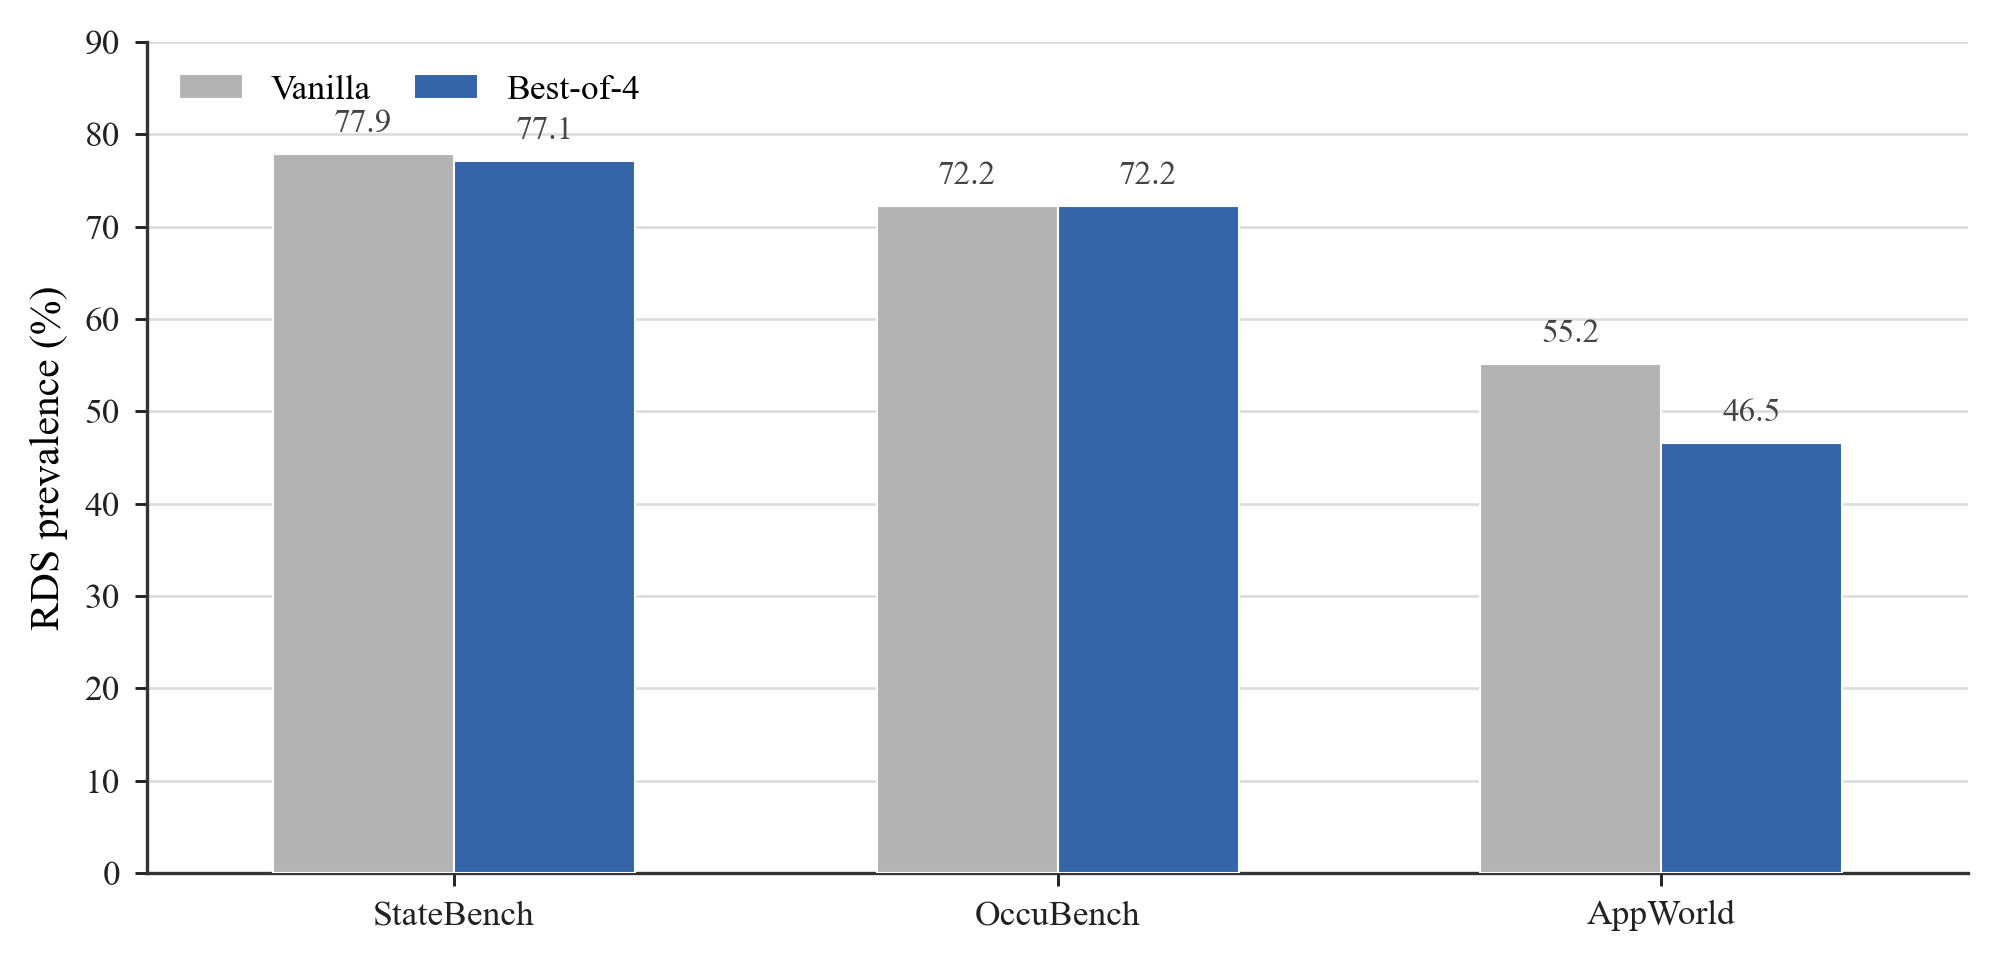
\includegraphics[width=\linewidth]{figures/baseline_rds.png}
\par\vspace{4pt}\raggedright\normalfont\normalsize
(b) RDS prevalence.\par
\end{minipage}
\caption{DeepSeek-v4.1-Flash: detected FRD (a) and public RDS evidence (b) under Vanilla and Best-of-4. Values are task-level percentages under the stated protocol. Missing FRD detection does not certify absence; RDS excludes final evaluator labels.}
\label{fig:frd-rds-distribution}
\end{figure}

\subsection{FRD and task completion}
We next test whether trajectories with detected FRD are associated with lower task success. Figure~\ref{fig:frd-conditioned-success} shows that under Vanilla, FRD-positive trajectories have lower success on StateBench, OccuBench, and AppWorld, with the clearest gap on StateBench, where success falls from 67.3\% to 27.5\%. Under Best-of-4, StateBench and OccuBench show the same direction, with StateBench falling from 74.1\% to 35.9\%; AppWorld is near parity and shows a small reversal under Best-of-4. The relationship is therefore descriptive under the current adjudication protocol rather than universal or causal. The complementary group means “FRD not detected by this protocol,” not verified absence. Together with the prevalence results above, this supports FRD as an offline harm indicator and RDS as a broader public signal available before the final outcome.

\begin{figure}[!htb]
\centering
\begin{minipage}[t]{0.46\linewidth}
\vspace{0pt}
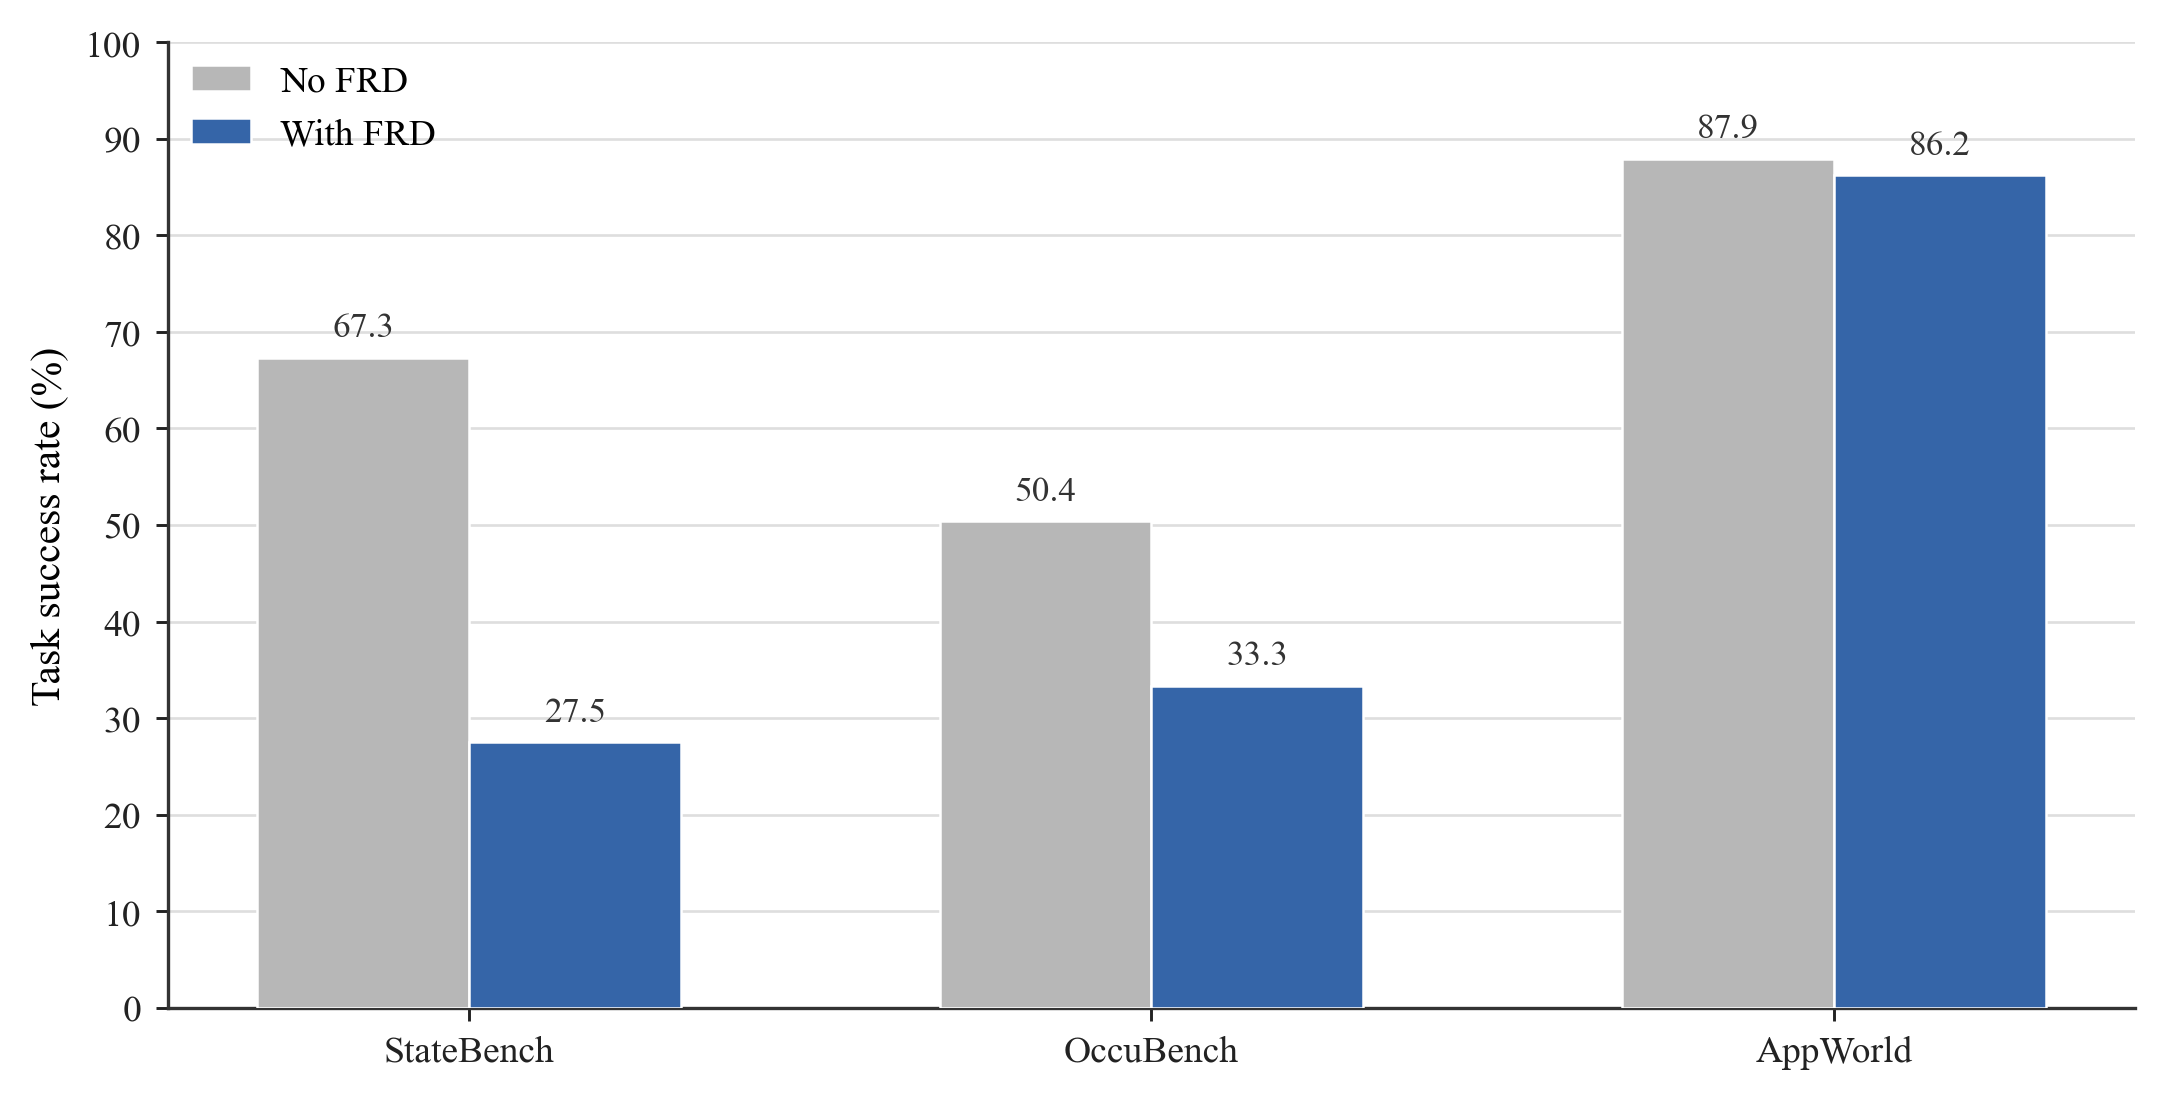
\includegraphics[width=\linewidth]{figures/frd_success_vanilla.png}
\par\vspace{4pt}\raggedright\normalfont\normalsize
(a) Vanilla.\par
\end{minipage}\hspace{0.02\linewidth}
\begin{minipage}[t]{0.46\linewidth}
\vspace{0pt}
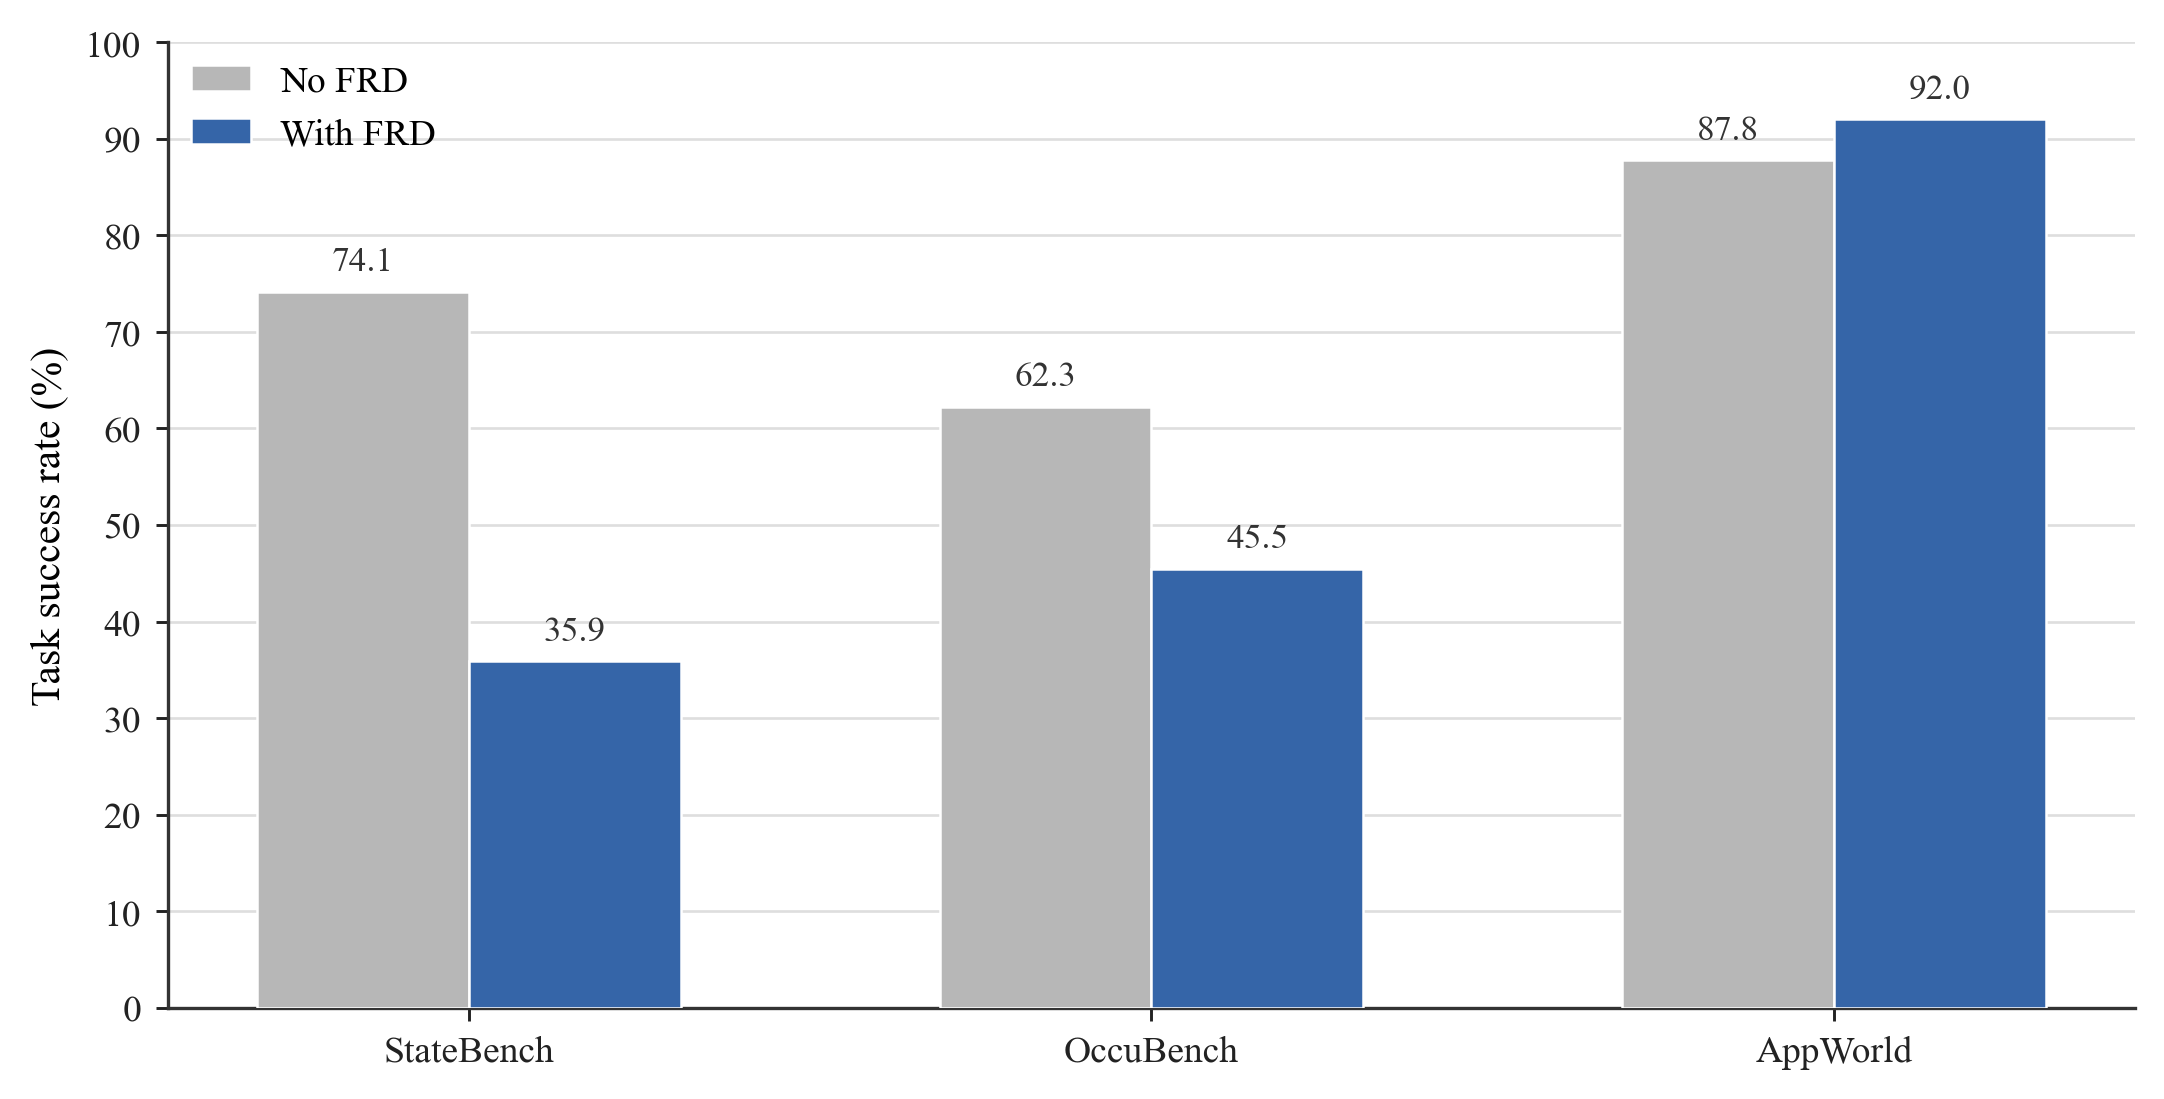
\includegraphics[width=\linewidth]{figures/frd_success_best4.png}
\par\vspace{4pt}\raggedright\normalfont\normalsize
(b) Best-of-4.\par
\end{minipage}
\caption{DeepSeek-v4.1-Flash task success with detected FRD versus no detected FRD under (a) Vanilla and (b) Best-of-4 on StateBench, OccuBench, and AppWorld. RDS prevalence appears in Figure~\ref{fig:frd-rds-distribution}(b).}
\label{fig:frd-conditioned-success}
\end{figure}

\section{RISE}
\label{sec:rise}
Figure~\ref{fig:frd-phenomenon} motivates using public recovery evidence to guide a new attempt. RISE performs this search over complete executions in fresh environments: it does not continue the incumbent environment or splice previously executed tool actions. The complete trajectory is the unit of generation and acceptance, public events are the unit of analysis and feedback, and a fresh environment is the boundary for each execution. The loop in Figure~\ref{fig:rise-overview} organizes three coupled updates in one accepted-incumbent search: RDS focuses the next proposal, public comparison selects the retained complete incumbent, and bilateral event feedback updates guidance for later rounds. The left panel provides the public event view, while the right panel shows the RISE controller. Together they form one procedure; benchmark-specific parsing and pseudocode appear in Appendix~\ref{app:implementation}.

\begin{figure}[!htb]
\centering
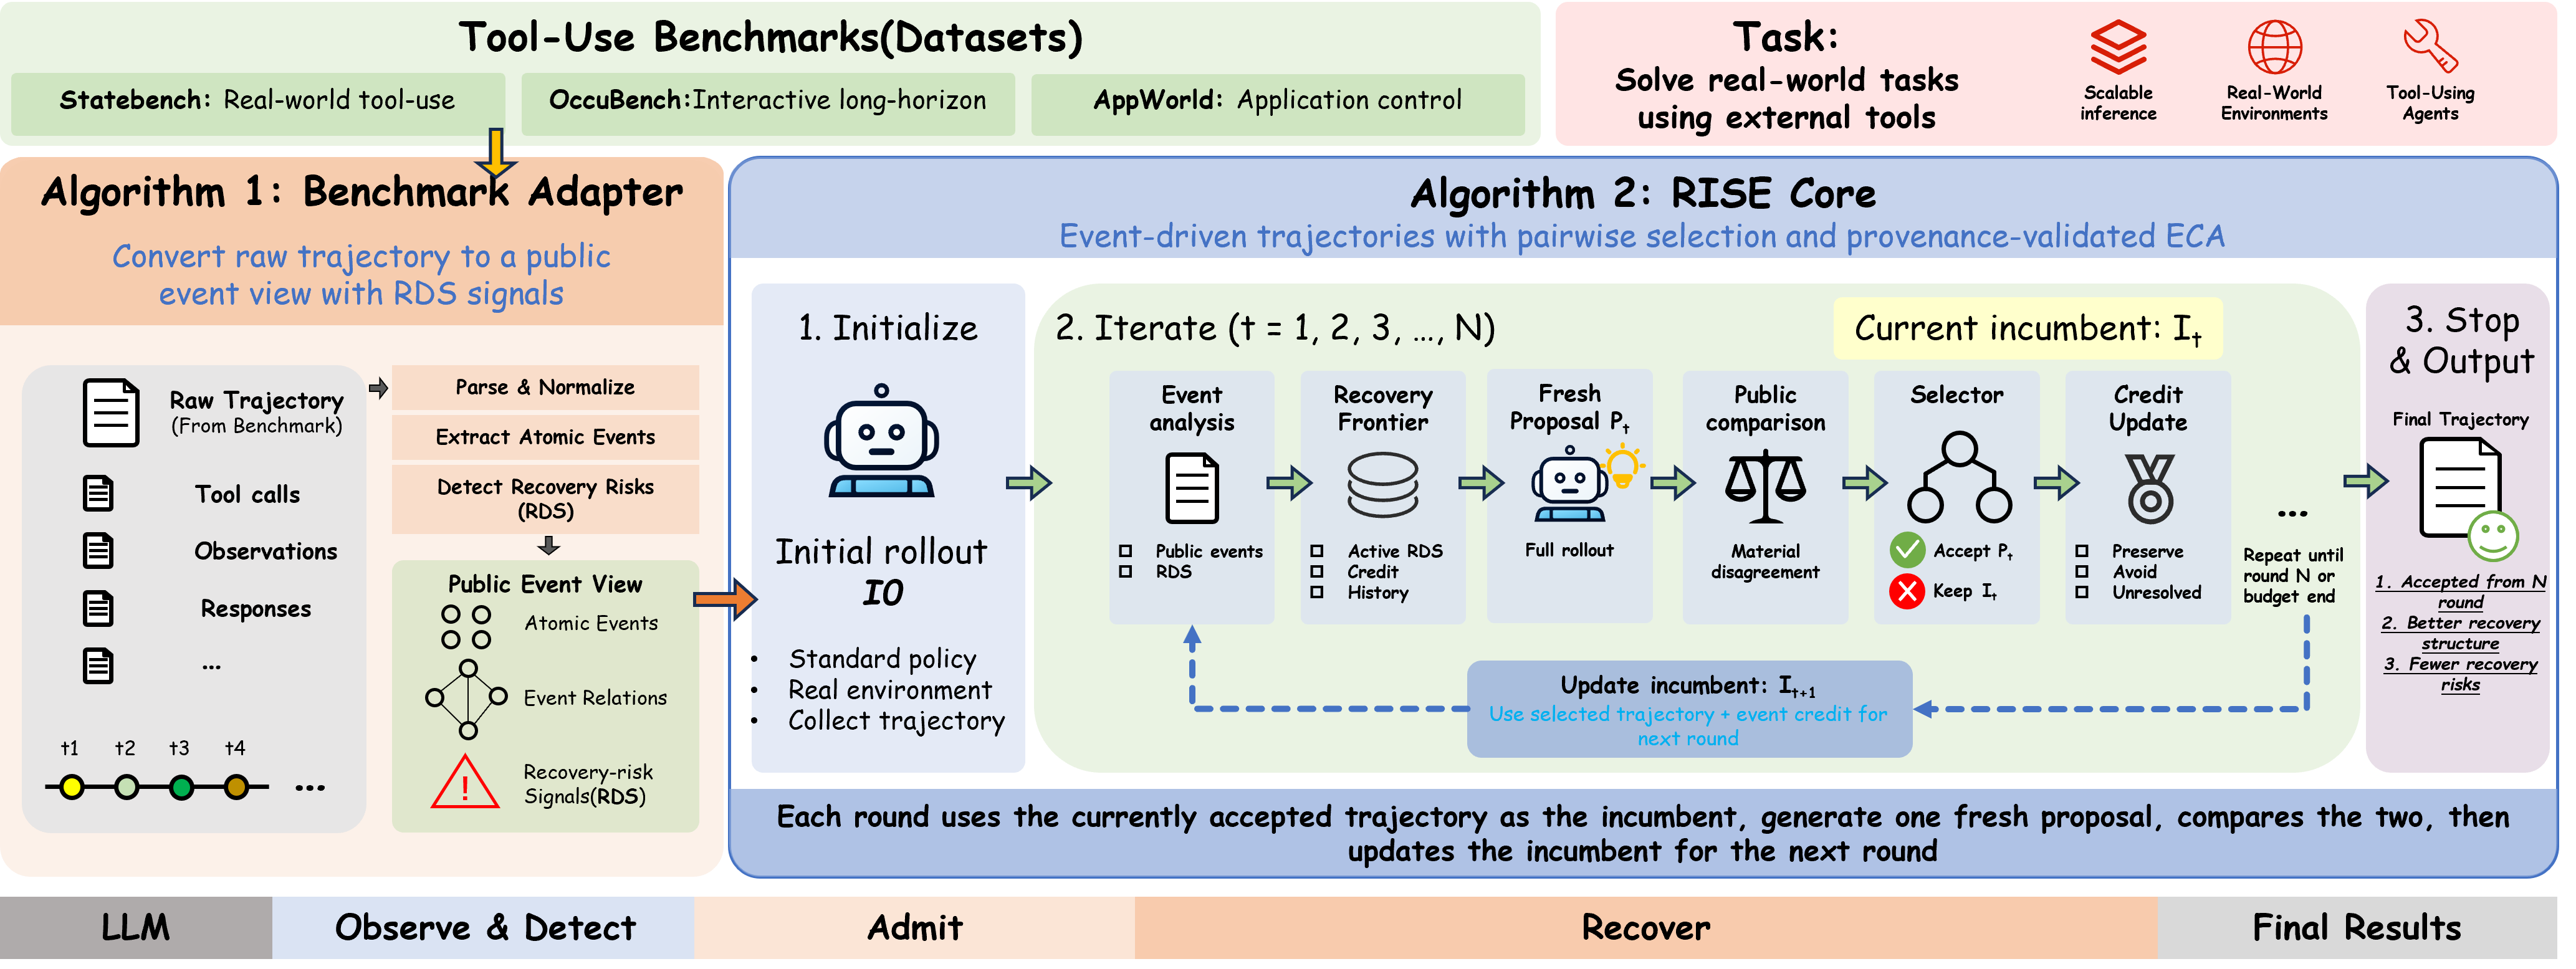
\includegraphics[width=1.00\linewidth]{figures/rise_method_overview.png}
\caption{RISE maps public interactions to events and RDS, builds a recovery frontier, generates a fresh complete proposal, and selects an incumbent under material disagreement. Bilateral preserve, avoid, and unresolved feedback guides subsequent rounds.}
\label{fig:rise-overview}
\end{figure}

\paragraph{Initialize the incumbent.}
RISE begins with an unguided Vanilla rollout $I_0$, empty event credit $C_0$, and initial permitted history $H_0$. The incumbent is the complete trajectory retained by the search, not a known correct answer. For a schedule of $N$ proposals, each round $t=0,\ldots,N-1$ executes the original task in a fresh environment. Cross-round guidance carries event structure, while each execution grounds object identifiers and argument values in its own environment.

\paragraph{Analyze events and construct the frontier.}
The event analysis maps a public trace through $A_b$ to $V_t=A_b(I_t)=(E_t,G_t,R_t)$. Here, $E_t$ contains atomic events with source identifiers and operation, argument, and result fields; $G_t$ contains supported transaction or recovery groups; and $R_t$ contains public Recovery-risk Disagreement Signal evidence. Grouping and risk extraction use only observations exposed by the benchmark. Recovery Frontier combines this evidence with event-credit feedback and history to form the guidance package $\mathcal{F}_t$ for Fresh Proposal. The frontier is a structured guidance package for the next complete execution, not a set of partially executed states:
\begin{equation}
\mathcal{F}_t=f_b(V_t,C_t,H_t),\qquad
P_t=\operatorname{FreshRollout}_{b,\theta}(x,\mathcal{F}_t).
\label{eq:frontier}
\end{equation}
The model $\theta$ then generates a complete proposal $P_t$. Current RDS determines the active recovery focus; an unresolved issue from earlier credit fills this role only when current risk evidence is absent. Preserve and avoid credit convey reusable structure, while permitted history stores abstracted comparison information. All online modules exclude hidden state, evaluator labels, and manual FRD annotations.

\paragraph{Compare public events and select a complete trajectory.}
The public-comparison block computes $D_t=d_b(A_b(I_t),A_b(P_t))$, a benchmark-specific material-disagreement predicate. StateBench compares transaction content and order; OccuBench uses its compatible event representation; AppWorld compares ordered API-signature lists. When $D_t=0$, RISE retains $I_t$ and skips candidate selection; only benchmark-defined non-comparison history updates are applied. Otherwise, the selector compares the two complete candidates through their public representations and either accepts $P_t$ or retains $I_t$. Its valid choice $q_t\in\{\mathrm{inc},\mathrm{prop}\}$ determines
\begin{equation}
I_{t+1}=\begin{cases}P_t,&D_t=1\ \text{and}\ q_t=\mathrm{prop},\\
I_t,&\text{otherwise}.\end{cases}
\label{eq:incumbent}
\end{equation}
The selector considers task coverage, grounding, action order, public effects, recovery, verification, and stopping. If it returns a fallback, RISE retains the incumbent and does not treat the fallback as a valid selected/rejected comparison for event credit. An execution error either exits or resumes according to the configured benchmark runner; it does not create event credit without a valid comparison.

\paragraph{Update event-credit feedback from both candidates.}
Let $V_t^s$ and $V_t^r$ denote the selected and rejected public event views. The Credit Update block applies event-credit feedback after a valid comparison:
\begin{equation}
C_{t+1}=u_b(V_t^s,V_t^r,D_t,q_t,C_t)
       =(C_{t+1}^{+},C_{t+1}^{-},z_{t+1}),
\label{eq:credit}
\end{equation}
where $C^+$ contains preserve structures, $C^-$ contains avoid structures, and $z$ is an unresolved issue. Preserve events originate from the selected side, and avoid events originate from the rejected side. Source validation checks these origins before structural projection removes candidate-specific literals. Credit supplies generation guidance without certifying event correctness or splicing actions from one candidate into another. StateBench derives credit deterministically from both event sets; OccuBench and AppWorld validate model-nominated event references. Appendix~\ref{app:implementation} details these differences.

Event credit can change even when the incumbent stays fixed. In StateBench, for example, an otherwise eligible ordinary event contributes to preserve when its shape is absent from the rejected side, while mutation and verification events follow an exception. Changing only the rejected candidate can therefore change the next guidance package. This is the role of the dashed feedback path in Figure~\ref{fig:rise-overview}: the next round receives both the accepted trajectory and credit derived from the two candidates.

\paragraph{Repeat and return the accepted trajectory.}
The Update incumbent feedback path carries $I_{t+1}$, $C_{t+1}$, and updated permitted history $H_{t+1}$ into the next recovery frontier. Algorithm~\ref{alg:rise} in Appendix~\ref{app:implementation} summarizes the process. A completed $N$-proposal schedule uses $K=N+1$ full rollouts. The default A/B/C/D schedule sets $N=3$ and $K=4$ only for exposition; A, B, C, and D are sequential candidate labels, not a restriction of RISE. The runner can configure any valid number $N$ of proposal rounds and its corresponding budget. Stop \& Output returns the final incumbent when the schedule ends or the configured budget is exhausted; it may originate in any round, including Vanilla.


\section{Experiments}
We report multi-model results on four benchmarks, comparing aggregate performance before analyzing the role of recovery guidance.
\subsection{Benchmarks}
We evaluate RISE on four complementary benchmarks. \textbf{STATE-Bench} is a stateful conversational tool-use benchmark covering Travel, Customer Support, and Shopping Assistant tasks. Version v0.8.1 contains 50 held-out tasks per category, for 150 tasks in total. Under the official protocol, PASS@1 is the average completion rate over five runs per task, PASS$^5$ is the fraction of tasks completed in all five runs, and UX is the mean user-experience score (1--5) over valid judged trajectories.

\textbf{AppWorld} evaluates persistent Python/API interactions across multiple applications. We use 585 tasks: Test-Normal contains 168 tasks and 56 scenario groups, and Test-Challenge contains 417 tasks and 139 scenario groups. Both splits report task-goal completion (TGC) and scenario-goal completion (SGC). TGC requires every test for an individual task to pass; SGC requires every task in a scenario group to pass.

\textbf{OccuBench} evaluates tool calling in professional settings. It contains 100 scenarios spanning ten occupational domains and 65 specialized domains, with 382 evaluation instances. We report task completion using PASS@1, the fraction of successful evaluation instances among the 382 instances. Its language-world-model simulator supplies tool responses and fault conditions, allowing the benchmark to test recovery under realistic occupational state changes.

\textbf{DeepPlanning Travel} evaluates travel planning under commonsense constraints and personalized requirements. Our evaluation includes 120 Chinese (ZH) and 120 English (EN) tasks. We report Delivery for plan delivery, Commonsense and Personalized for satisfaction of the corresponding requirements, and Composite for overall planning performance, separately for each language.

\subsection{Protocol and results}
Vanilla uses one rollout; Best-of-4 selects from four candidates. All four benchmarks report the OAgents Best-of-4 comparison; the DeepSeek AppWorld configuration shares initial candidate A with Vanilla. RISE uses a matched full-rollout budget: one initial trajectory followed by three guided proposals. This matches complete executions, not total compute, because RISE also performs public-event analysis, candidate comparison, and feedback construction. DeepSeek-v4.1-Flash, Qwen3.8-Max, and GPT-5.6-Sol cover all four benchmarks. Tasks, tools, simulators, and evaluators are fixed across methods within each evaluation cohort. Online decisions use only public traces, excluding evaluator labels, hidden state, and gold actions. Tables~\ref{tab:statebench-models}--\ref{tab:deepplanning-models} place Vanilla and Best-of-4 above RISE; pairs below RISE report differences from these baselines in that order.

\paragraph{Stateful conversational tool use on StateBench.} StateBench tests whether LLMs can complete tasks through stateful conversations and tool calls. Table~\ref{tab:statebench-models} shows that RISE improves PASS@1, PASS$^5$, and UX over both baselines for all three models. Qwen3.8-Max and GPT-5.6-Sol each gain 5.33 percentage points in PASS@1 over Best-of-4; GPT-5.6-Sol reaches 83.33\% PASS@1 and 56.00\% PASS$^5$. The improvements extend from average completion to consistency across repeated runs and user experience.

\begin{table}[!htb]
\centering
\scriptsize
\setlength{\tabcolsep}{2.5pt}
\renewcommand{\arraystretch}{1.12}
\caption{STATE-Bench results. Parenthesized pairs below RISE compare with Vanilla and Best-of-4, in that order. Differences use reported scores: percentage points for PASS and score units for UX.}
\label{tab:statebench-models}
\begin{tabular*}{\linewidth}{@{\extracolsep{\fill}}llccc@{}}
\toprule
Setting & Base LLM & \shortstack{PASS@1\\(\%) $\uparrow$} & \shortstack{PASS$^5$\\(\%) $\uparrow$} & \shortstack{UX\\(1--5) $\uparrow$} \\
\midrule
Vanilla & deepseek-v4.1-flash & 65.20 & 38.67 & 3.9709 \\
Vanilla & qwen3.8-max & 69.33 & 41.33 & 4.0217 \\
Vanilla & gpt-5.6-sol & 71.33 & 42.00 & 4.0658 \\
\midrule
Best-of-4 & deepseek-v4.1-flash & 72.13 & 46.67 & 4.1428 \\
Best-of-4 & qwen3.8-max & 76.00 & 49.33 & 4.1893 \\
Best-of-4 & gpt-5.6-sol & 78.00 & 50.67 & 4.2374 \\
\midrule
\textbf{RISE} & deepseek-v4.1-flash & \shortstack[c]{\textbf{72.67}\\[-1pt]{\scriptsize $(+7.47,+0.54)$}} & \shortstack[c]{\textbf{48.67}\\[-1pt]{\scriptsize $(+10.00,+2.00)$}} & \shortstack[c]{\textbf{4.1499}\\[-1pt]{\scriptsize $(+0.1790,+0.0071)$}} \\
\textbf{RISE} & qwen3.8-max & \shortstack[c]{\textbf{81.33}\\[-1pt]{\scriptsize $(+12.00,+5.33)$}} & \shortstack[c]{\textbf{54.67}\\[-1pt]{\scriptsize $(+13.34,+5.34)$}} & \shortstack[c]{\textbf{4.3512}\\[-1pt]{\scriptsize $(+0.3295,+0.1619)$}} \\
\textbf{RISE} & gpt-5.6-sol & \shortstack[c]{\textbf{83.33}\\[-1pt]{\scriptsize $(+12.00,+5.33)$}} & \shortstack[c]{\textbf{56.00}\\[-1pt]{\scriptsize $(+14.00,+5.33)$}} & \shortstack[c]{\textbf{4.3981}\\[-1pt]{\scriptsize $(+0.3323,+0.1607)$}} \\
\bottomrule
\end{tabular*}
\end{table}

\paragraph{Cross-application task completion on AppWorld.} AppWorld requires LLMs to coordinate Python and API interactions across applications in a persistent environment. Table~\ref{tab:appworld-models} reports higher task and scenario completion for every model on both test splits. On Test-Challenge, Qwen3.8-Max and GPT-5.6-Sol each improve SGC by 7.91 percentage points over Best-of-4. Because SGC requires all tasks in a scenario group to succeed, these gains extend beyond isolated task completion to satisfying the stricter group-level criterion.

\begin{table}[!htb]
\centering
\scriptsize
\setlength{\tabcolsep}{2pt}
\renewcommand{\arraystretch}{1.12}
\caption{AppWorld percentages and success counts. Test-Normal has 168 tasks/56 scenario groups; Test-Challenge has 417/139. RISE differences from Vanilla and Best-of-4 use unrounded counts (percentage points).}
\label{tab:appworld-models}
\begin{tabular*}{\linewidth}{@{\extracolsep{\fill}}llcccc@{}}
\toprule
\multirow{2}{*}{Setting} & \multirow{2}{*}{Base LLM} & \multicolumn{2}{c}{Test-Normal} & \multicolumn{2}{c}{Test-Challenge} \\
\cmidrule(lr){3-4}\cmidrule(l){5-6}
 &  & TGC (\%) $\uparrow$ & SGC (\%) $\uparrow$ & TGC (\%) $\uparrow$ & SGC (\%) $\uparrow$ \\
\midrule
Vanilla & deepseek-v4.1-flash & 91.07 (153/168) & 80.36 (45/56) & 87.77 (366/417) & 75.54 (105/139) \\
Vanilla & qwen3.8-max & 91.07 (153/168) & 82.14 (46/56) & 89.93 (375/417) & 79.14 (110/139) \\
Vanilla & gpt-5.6-sol & 92.26 (155/168) & 83.93 (47/56) & 90.65 (378/417) & 80.58 (112/139) \\
\midrule
Best-of-4 & deepseek-v4.1-flash & 91.07 (153/168) & 82.14 (46/56) & 88.01 (367/417) & 77.70 (108/139) \\
Best-of-4 & qwen3.8-max & 92.26 (155/168) & 83.93 (47/56) & 90.41 (377/417) & 81.29 (113/139) \\
Best-of-4 & gpt-5.6-sol & 93.45 (157/168) & 85.71 (48/56) & 91.13 (380/417) & 82.73 (115/139) \\
\midrule
\textbf{RISE} & deepseek-v4.1-flash & \shortstack[c]{\textbf{92.26 (155/168)}\\[-1pt]{\scriptsize $(+1.19,+1.19)$}} & \shortstack[c]{\textbf{85.71 (48/56)}\\[-1pt]{\scriptsize $(+5.36,+3.57)$}} & \shortstack[c]{\textbf{89.69 (374/417)}\\[-1pt]{\scriptsize $(+1.92,+1.68)$}} & \shortstack[c]{\textbf{82.01 (114/139)}\\[-1pt]{\scriptsize $(+6.47,+4.32)$}} \\
\textbf{RISE} & qwen3.8-max & \shortstack[c]{\textbf{96.43 (162/168)}\\[-1pt]{\scriptsize $(+5.36,+4.17)$}} & \shortstack[c]{\textbf{91.07 (51/56)}\\[-1pt]{\scriptsize $(+8.93,+7.14)$}} & \shortstack[c]{\textbf{94.96 (396/417)}\\[-1pt]{\scriptsize $(+5.04,+4.56)$}} & \shortstack[c]{\textbf{89.21 (124/139)}\\[-1pt]{\scriptsize $(+10.07,+7.91)$}} \\
\textbf{RISE} & gpt-5.6-sol & \shortstack[c]{\textbf{97.62 (164/168)}\\[-1pt]{\scriptsize $(+5.36,+4.17)$}} & \shortstack[c]{\textbf{92.86 (52/56)}\\[-1pt]{\scriptsize $(+8.93,+7.14)$}} & \shortstack[c]{\textbf{95.68 (399/417)}\\[-1pt]{\scriptsize $(+5.04,+4.56)$}} & \shortstack[c]{\textbf{90.65 (126/139)}\\[-1pt]{\scriptsize $(+10.07,+7.91)$}} \\
\bottomrule
\end{tabular*}
\end{table}

\paragraph{Professional tool use on OccuBench.} OccuBench evaluates tool use in professional scenarios. Table~\ref{tab:occubench-models} shows that RISE improves PASS@1 over both baselines for all three models, with gains over Best-of-4 ranging from 1.57 to 6.02 percentage points. GPT-5.6-Sol achieves the highest PASS@1 of 76.70\%, improving by 17.02 points over Vanilla and 6.02 points over Best-of-4. The consistent direction across models supports the usefulness of recovery-guided rollouts in professional tool-use tasks.

\begin{table}[!htb]
\centering
\scriptsize
\setlength{\tabcolsep}{2.5pt}
\renewcommand{\arraystretch}{1.12}
\caption{OccuBench PASS@1 on 382 instances. Pairs below RISE give percentage-point differences from Vanilla and Best-of-4, computed from unrounded success rates.}
\label{tab:occubench-models}
\begin{tabular*}{\linewidth}{@{\extracolsep{\fill}}llc@{}}
\toprule
Setting & Base LLM & PASS@1 (\%) $\uparrow$ \\
\midrule
Vanilla & deepseek-v4.1-flash & 49.74 \\
Vanilla & qwen3.8-max & 57.85 \\
Vanilla & gpt-5.6-sol & 59.69 \\
\midrule
Best-of-4 & deepseek-v4.1-flash & 61.78 \\
Best-of-4 & qwen3.8-max & 68.85 \\
Best-of-4 & gpt-5.6-sol & 70.68 \\
\midrule
\textbf{RISE} & deepseek-v4.1-flash & \shortstack[c]{\textbf{63.35}\\[-1pt]{\scriptsize $(+13.61,+1.57)$}} \\
\textbf{RISE} & qwen3.8-max & \shortstack[c]{\textbf{74.61}\\[-1pt]{\scriptsize $(+16.75,+5.76)$}} \\
\textbf{RISE} & gpt-5.6-sol & \shortstack[c]{\textbf{76.70}\\[-1pt]{\scriptsize $(+17.02,+6.02)$}} \\
\bottomrule
\end{tabular*}
\end{table}
\paragraph{Travel planning on DeepPlanning.} DeepPlanning Travel evaluates plan delivery alongside commonsense and personalized requirements. Table~\ref{tab:deepplanning-models} shows improvements over both baselines on all four metrics for every model in both languages. Composite gains over Best-of-4 range from 5.73 to 5.92 percentage points, with GPT-5.6-Sol reaching 48.43\% on the English cohort. Improvements in Commonsense and Personalized scores alongside Delivery indicate that the gains extend beyond producing a plan to meeting its evaluated requirements.

\begin{table}[!htb]
\centering
\scriptsize
\setlength{\tabcolsep}{1.6pt}
\renewcommand{\arraystretch}{1.12}
\caption{DeepPlanning Travel scores (\%) for Chinese (ZH) and English (EN), 120 tasks each. RISE differences from Vanilla and Best-of-4 use percentage points; Delivery uses unrounded counts. Bold marks the best score within each model--language cohort.}
\label{tab:deepplanning-models}
\begin{tabular*}{\linewidth}{@{\extracolsep{\fill}}lllcccc@{}}
\toprule
Setting & Base LLM & Cohort & \shortstack{Delivery\\$\uparrow$} & \shortstack{Common-\\sense $\uparrow$} & \shortstack{Personalized\\$\uparrow$} & \shortstack{Composite\\$\uparrow$} \\
\midrule
Vanilla & deepseek-v4.1-flash & ZH (120) & 85.83 (103/120) & 39.27 & 27.94 & 32.71 \\
Vanilla & deepseek-v4.1-flash & EN (120) & 90.83 (109/120) & 45.62 & 25.83 & 35.84 \\
Vanilla & qwen3.8-max & ZH (120) & 89.17 (107/120) & 41.63 & 29.73 & 34.58 \\
Vanilla & qwen3.8-max & EN (120) & 94.17 (113/120) & 47.86 & 27.64 & 37.79 \\
Vanilla & gpt-5.6-sol & ZH (120) & 90.83 (109/120) & 42.75 & 30.58 & 35.66 \\
Vanilla & gpt-5.6-sol & EN (120) & 95.00 (114/120) & 48.71 & 28.37 & 38.62 \\
\midrule
Best-of-4 & deepseek-v4.1-flash & ZH (120) & 89.17 (107/120) & 43.18 & 30.86 & 36.42 \\
Best-of-4 & deepseek-v4.1-flash & EN (120) & 93.33 (112/120) & 49.37 & 28.94 & 39.58 \\
Best-of-4 & qwen3.8-max & ZH (120) & 92.50 (111/120) & 45.82 & 32.85 & 38.47 \\
Best-of-4 & qwen3.8-max & EN (120) & 95.83 (115/120) & 51.74 & 30.92 & 41.63 \\
Best-of-4 & gpt-5.6-sol & ZH (120) & 93.33 (112/120) & 46.91 & 33.72 & 39.58 \\
Best-of-4 & gpt-5.6-sol & EN (120) & 96.67 (116/120) & 52.63 & 31.59 & 42.51 \\
\midrule
\textbf{RISE} & deepseek-v4.1-flash & ZH (120) & \shortstack[c]{\textbf{95.00 (114/120)}\\[-1pt]{\scriptsize $(+9.17,+5.83)$}} & \shortstack[c]{\textbf{49.86}\\[-1pt]{\scriptsize $(+10.59,+6.68)$}} & \shortstack[c]{\textbf{36.41}\\[-1pt]{\scriptsize $(+8.47,+5.55)$}} & \shortstack[c]{\textbf{42.18}\\[-1pt]{\scriptsize $(+9.47,+5.76)$}} \\
\textbf{RISE} & deepseek-v4.1-flash & EN (120) & \shortstack[c]{\textbf{97.50 (117/120)}\\[-1pt]{\scriptsize $(+6.67,+4.17)$}} & \shortstack[c]{\textbf{56.13}\\[-1pt]{\scriptsize $(+10.51,+6.76)$}} & \shortstack[c]{\textbf{34.28}\\[-1pt]{\scriptsize $(+8.45,+5.34)$}} & \shortstack[c]{\textbf{45.31}\\[-1pt]{\scriptsize $(+9.47,+5.73)$}} \\
\textbf{RISE} & qwen3.8-max & ZH (120) & \shortstack[c]{\textbf{96.67 (116/120)}\\[-1pt]{\scriptsize $(+7.50,+4.17)$}} & \shortstack[c]{\textbf{51.83}\\[-1pt]{\scriptsize $(+10.20,+6.01)$}} & \shortstack[c]{\textbf{38.27}\\[-1pt]{\scriptsize $(+8.54,+5.42)$}} & \shortstack[c]{\textbf{44.26}\\[-1pt]{\scriptsize $(+9.68,+5.79)$}} \\
\textbf{RISE} & qwen3.8-max & EN (120) & \shortstack[c]{\textbf{98.33 (118/120)}\\[-1pt]{\scriptsize $(+4.17,+2.50)$}} & \shortstack[c]{\textbf{58.41}\\[-1pt]{\scriptsize $(+10.55,+6.67)$}} & \shortstack[c]{\textbf{36.53}\\[-1pt]{\scriptsize $(+8.89,+5.61)$}} & \shortstack[c]{\textbf{47.52}\\[-1pt]{\scriptsize $(+9.73,+5.89)$}} \\
\textbf{RISE} & gpt-5.6-sol & ZH (120) & \shortstack[c]{\textbf{97.50 (117/120)}\\[-1pt]{\scriptsize $(+6.67,+4.17)$}} & \shortstack[c]{\textbf{52.94}\\[-1pt]{\scriptsize $(+10.19,+6.03)$}} & \shortstack[c]{\textbf{39.18}\\[-1pt]{\scriptsize $(+8.60,+5.46)$}} & \shortstack[c]{\textbf{45.37}\\[-1pt]{\scriptsize $(+9.71,+5.79)$}} \\
\textbf{RISE} & gpt-5.6-sol & EN (120) & \shortstack[c]{\textbf{99.17 (119/120)}\\[-1pt]{\scriptsize $(+4.17,+2.50)$}} & \shortstack[c]{\textbf{59.26}\\[-1pt]{\scriptsize $(+10.55,+6.63)$}} & \shortstack[c]{\textbf{37.35}\\[-1pt]{\scriptsize $(+8.98,+5.76)$}} & \shortstack[c]{\textbf{48.43}\\[-1pt]{\scriptsize $(+9.81,+5.92)$}} \\
\bottomrule
\end{tabular*}
\end{table}

Taken together, the four benchmarks show a consistent improvement trend across all three evaluated models, with gains varying by task and model. Under the same complete-rollout budget as Best-of-4, RISE improves the reported outcomes across conversational tool use, application interaction, professional tasks, and travel planning.

\section{Analysis}
We organize the analysis around four questions: which RISE components matter, whether the mechanism succeeds in a concrete case, whether RISE reduces final FRD and RDS prevalence, and whether it improves matched risk-positive cohorts. The quantitative analyses in Sections~5.3 and~5.4 use DeepSeek-v4.1-Flash.

\subsection{Ablations}
We first isolate the three guidance choices in RISE on 382 OccuBench instances. \textbf{No RDS focus} removes the explicit recovery focus supplied by the current Recovery-risk Disagreement Signal while retaining public events and other feedback. \textbf{No event-credit feedback} retains complete-candidate comparison and selection but blocks event-credit feedback from subsequent executions. \textbf{Pairwise summary} replaces event-credit feedback with a summary of the two public candidates. Vanilla and OAgents Best-of-4 are reference points; all conditions use the same task manifest, model, selector budget, and evaluation protocol.

\begin{table}[!htb]
\caption{OccuBench ablations on 382 evaluation instances. The last column reports the difference from full RISE in percentage points; negative values indicate a drop from full RISE.}
\label{tab:ablations}
\centering
\small
\begin{tabular}{lcc}
\toprule
Method & PASS@1 (\%) & Difference from Full RISE (pp) \\
\midrule
Vanilla & 49.74 & $-13.61$ \\
OAgents Best-of-4 & 61.78 & $-1.57$ \\
\textbf{RISE (Full)} & \textbf{63.35} & -- \\
No RDS focus & 53.14 & $-10.21$ \\
No event-credit feedback & 57.07 & $-6.28$ \\
Pairwise summary & 60.73 & $-2.62$ \\
\bottomrule
\end{tabular}
\end{table}

The complete RISE configuration reaches 63.35\% PASS@1, improving over Vanilla by 13.61 points and over OAgents Best-of-4 by 1.57 points. Each ablation is lower than full RISE, supporting complementary roles within the coupled guidance process rather than two independent controllers.

\paragraph{Explicit recovery focus.} Removing the current RDS focus lowers PASS@1 to 53.14\%, a 10.21-point drop from full RISE and the largest degradation among the variants. Public events and other feedback remain available in this condition, so the result indicates that a concrete recovery target adds information beyond the raw trajectory. RDS therefore does more than flag an anomaly: it identifies which unresolved issue the next complete rollout should recheck. This ablation isolates the use of the current risk signal and should not be interpreted as removing all RDS evidence from the system.

\paragraph{Cross-round event feedback.} Blocking event-credit feedback lowers PASS@1 to 57.07\%, 6.28 points below full RISE, even though candidate comparison and acceptance are unchanged. Candidate selection determines which complete trajectory becomes the incumbent, whereas event feedback tells the next rollout which structures to preserve, avoid, or revisit. The drop therefore supports an incremental role for carrying comparison evidence across rounds. It measures the feedback channel as a whole and does not separately attribute gains to preserve, avoid, or unresolved-issue credit.

\paragraph{Event credit versus pairwise summary.} Replacing event credit with a summary of the two candidates yields 60.73\% PASS@1. The summary is 3.66 points above the no-feedback variant, showing that generic comparison information can still help, but it remains 2.62 points below full RISE. The result suggests that feedback content and organization matter in addition to the presence of a feedback channel. Overall, RISE benefits from identifying a concrete recovery focus and from converting bilateral comparison into guidance for the next rollout.

\subsection{A verified intervention case}
Figure~\ref{fig:rise-recovery-case} traces the subsequent execution on the AppWorld task used in the case study. The first two pairwise comparisons retain baseline A: PLV(A,B) keeps A and PLV(A,C) keeps A. Candidate D receives a public frontier targeting A50 and a generic FAILURE\_RECOVERY instruction to re-ground the failed target and its preconditions. D starts in a fresh environment. It initially repeats unauthenticated reads, then consults the show\_drafts specification at D11 and supplies access\_token at D12. D continues checking threads and handling execution errors, processes remaining drafts during D14--D20, and completes the task at D21; the official evaluation reports 4/4 checks passed. The final comparison selects D. A, B, C, and D are only sequential labels for this illustrated schedule; RISE supports any configured number $N$ of proposal rounds. The case demonstrates a successful intervention, but does not isolate the causal contribution of one module.

\begin{figure}[!htb]
\centering
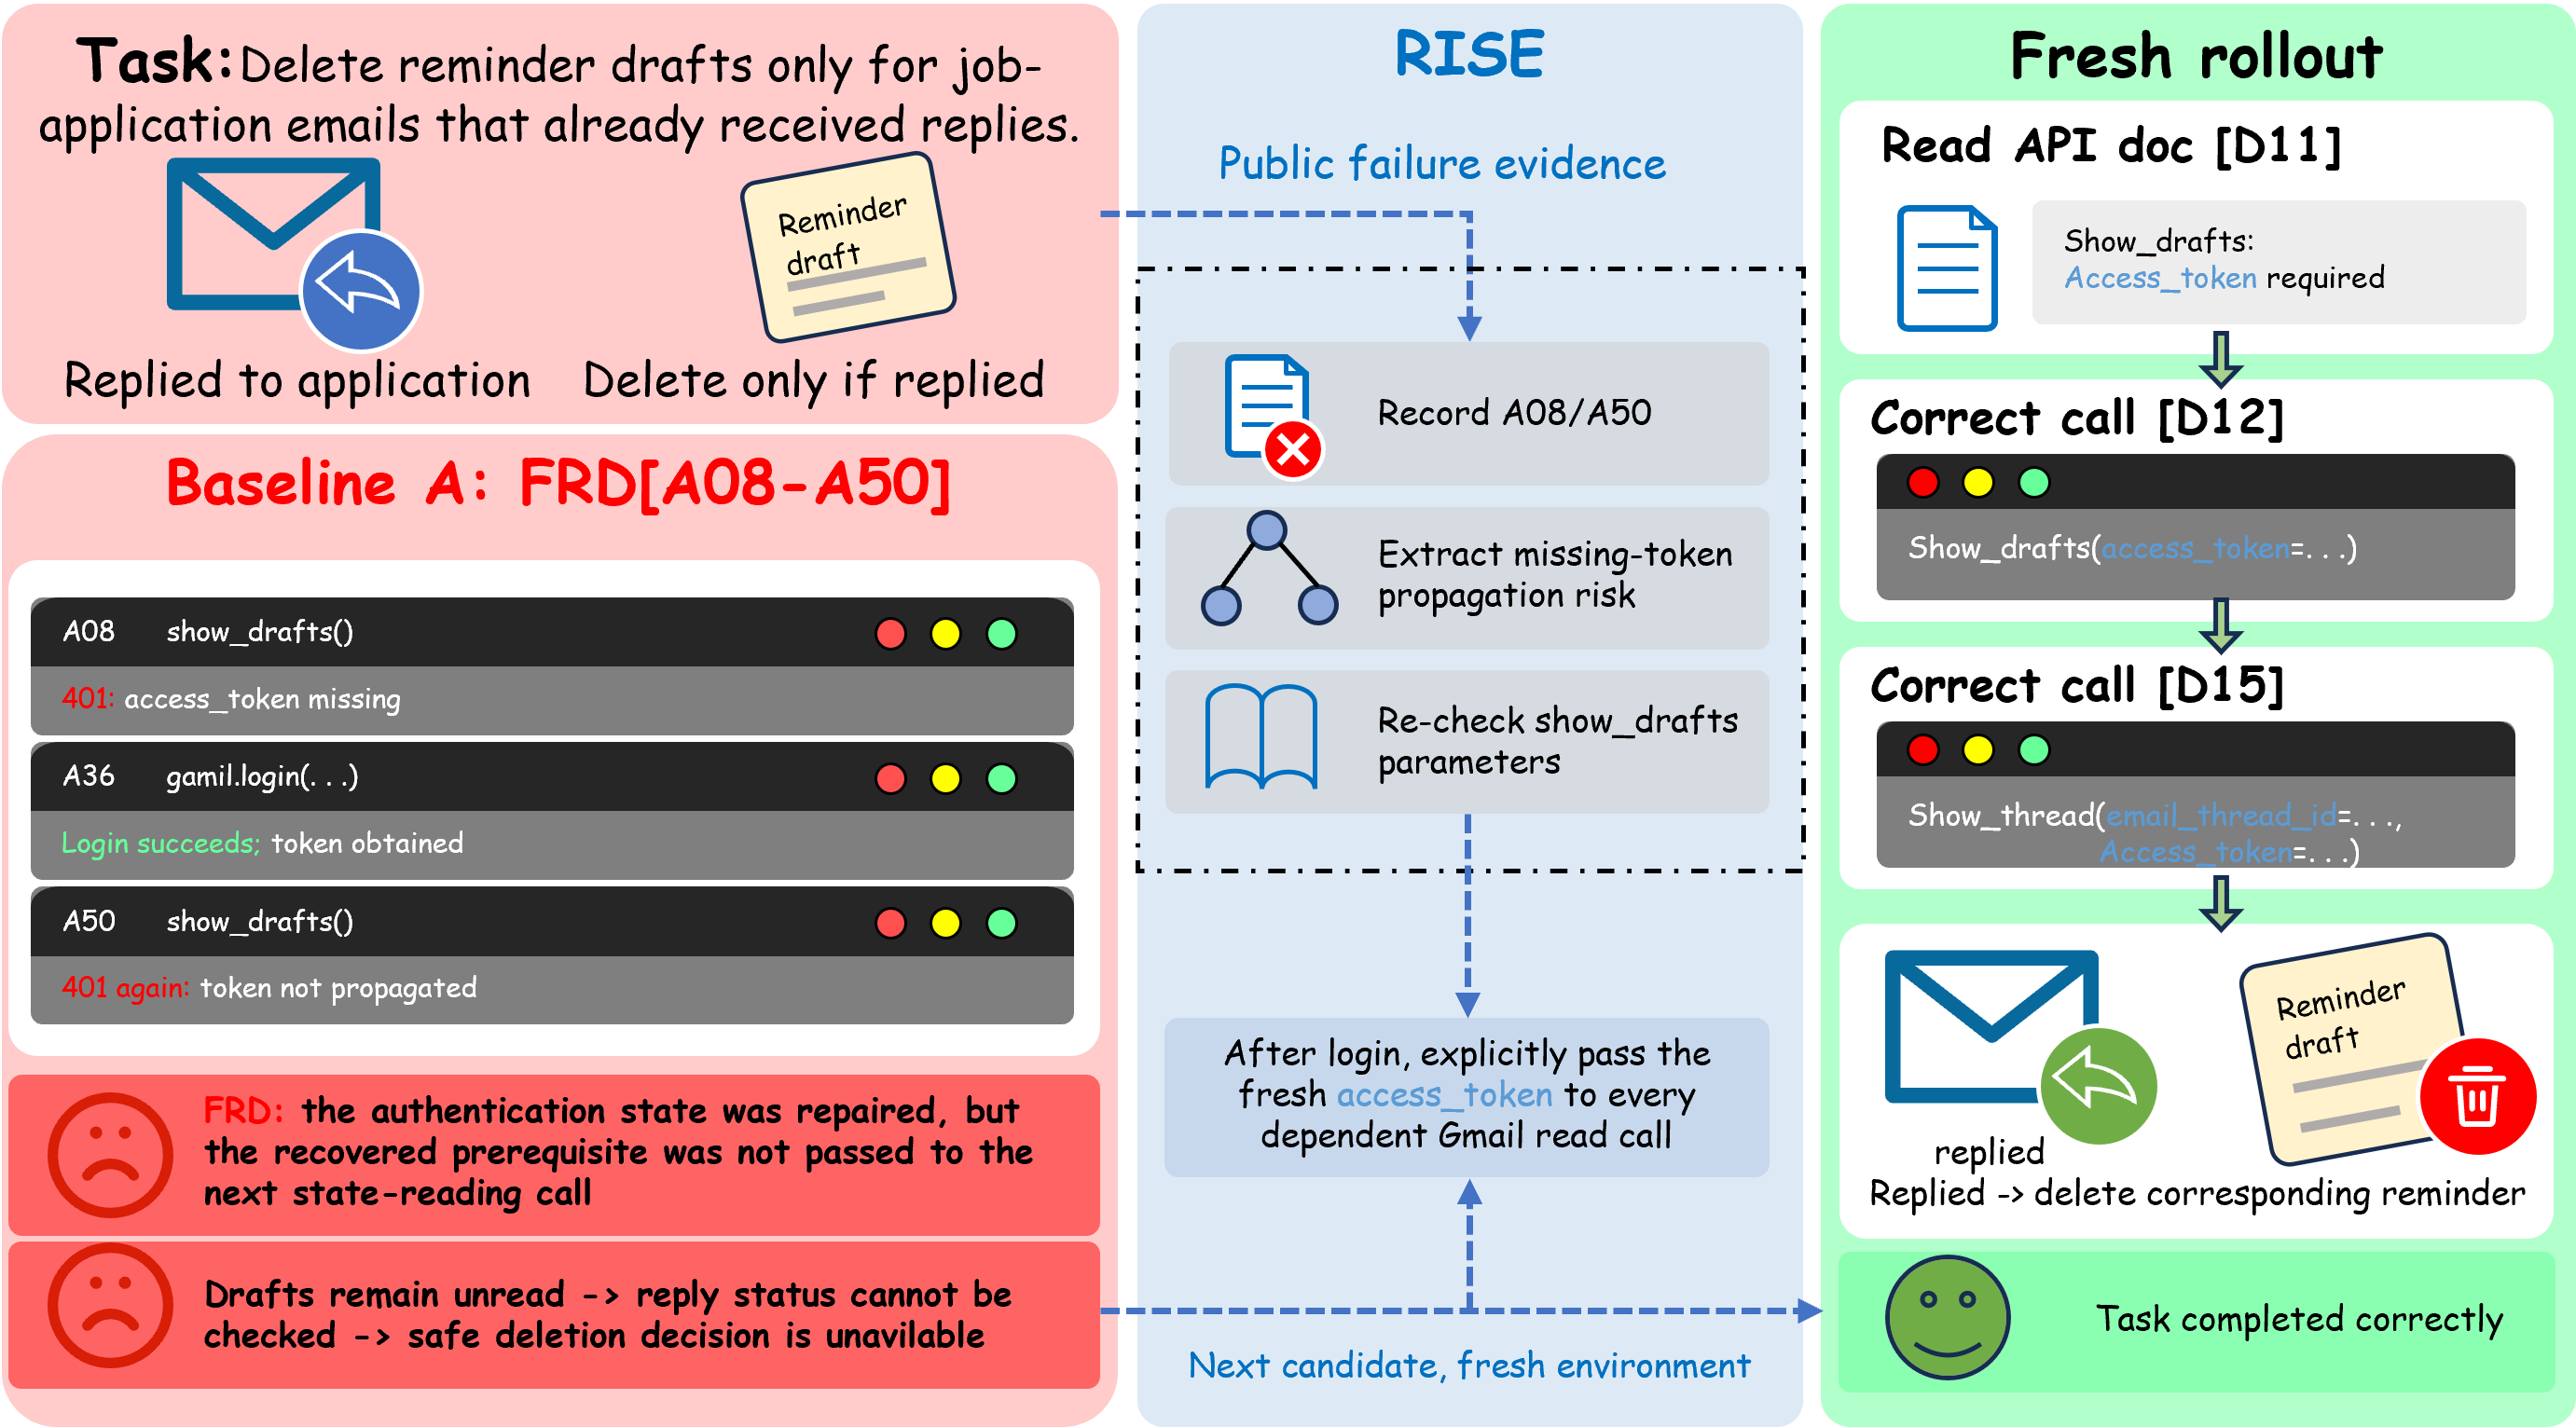
\includegraphics[width=0.85\linewidth]{figures/rise_recovery_case.png}
\caption{AppWorld intervention case. D resolves draft access at D12, passes official checks, and is selected. Guidance paraphrases the A50 frontier; intermediate PLV(A,B)/PLV(A,C) comparisons and D retries are omitted. This is a fresh rollout, not an in-place repair.}
\label{fig:rise-recovery-case}
\end{figure}

\subsection{Final FRD and Recovery-risk Disagreement Signal prevalence}
Figure~\ref{fig:analysis-frd-rds} shows that, among final selected trajectories from DeepSeek-v4.1-Flash, RISE lowers detected FRD and RDS prevalence across the three benchmarks. The largest change is on AppWorld: detected FRD drops from 7.0\% under Vanilla to 1.7\% under RISE (5.3 points), while RDS drops from 55.2\% to 26.4\% (28.8 points). StateBench also shows a clear reduction, and OccuBench shows a smaller reduction in the same direction. The two panels are consistent with the mechanism: public recovery evidence helps avoid repeated high-risk structures and reduces trajectories that end with unresolved recovery risk. 
\begin{figure}[!htb]
\centering
\begin{minipage}[t]{0.46\linewidth}
\vspace{0pt}
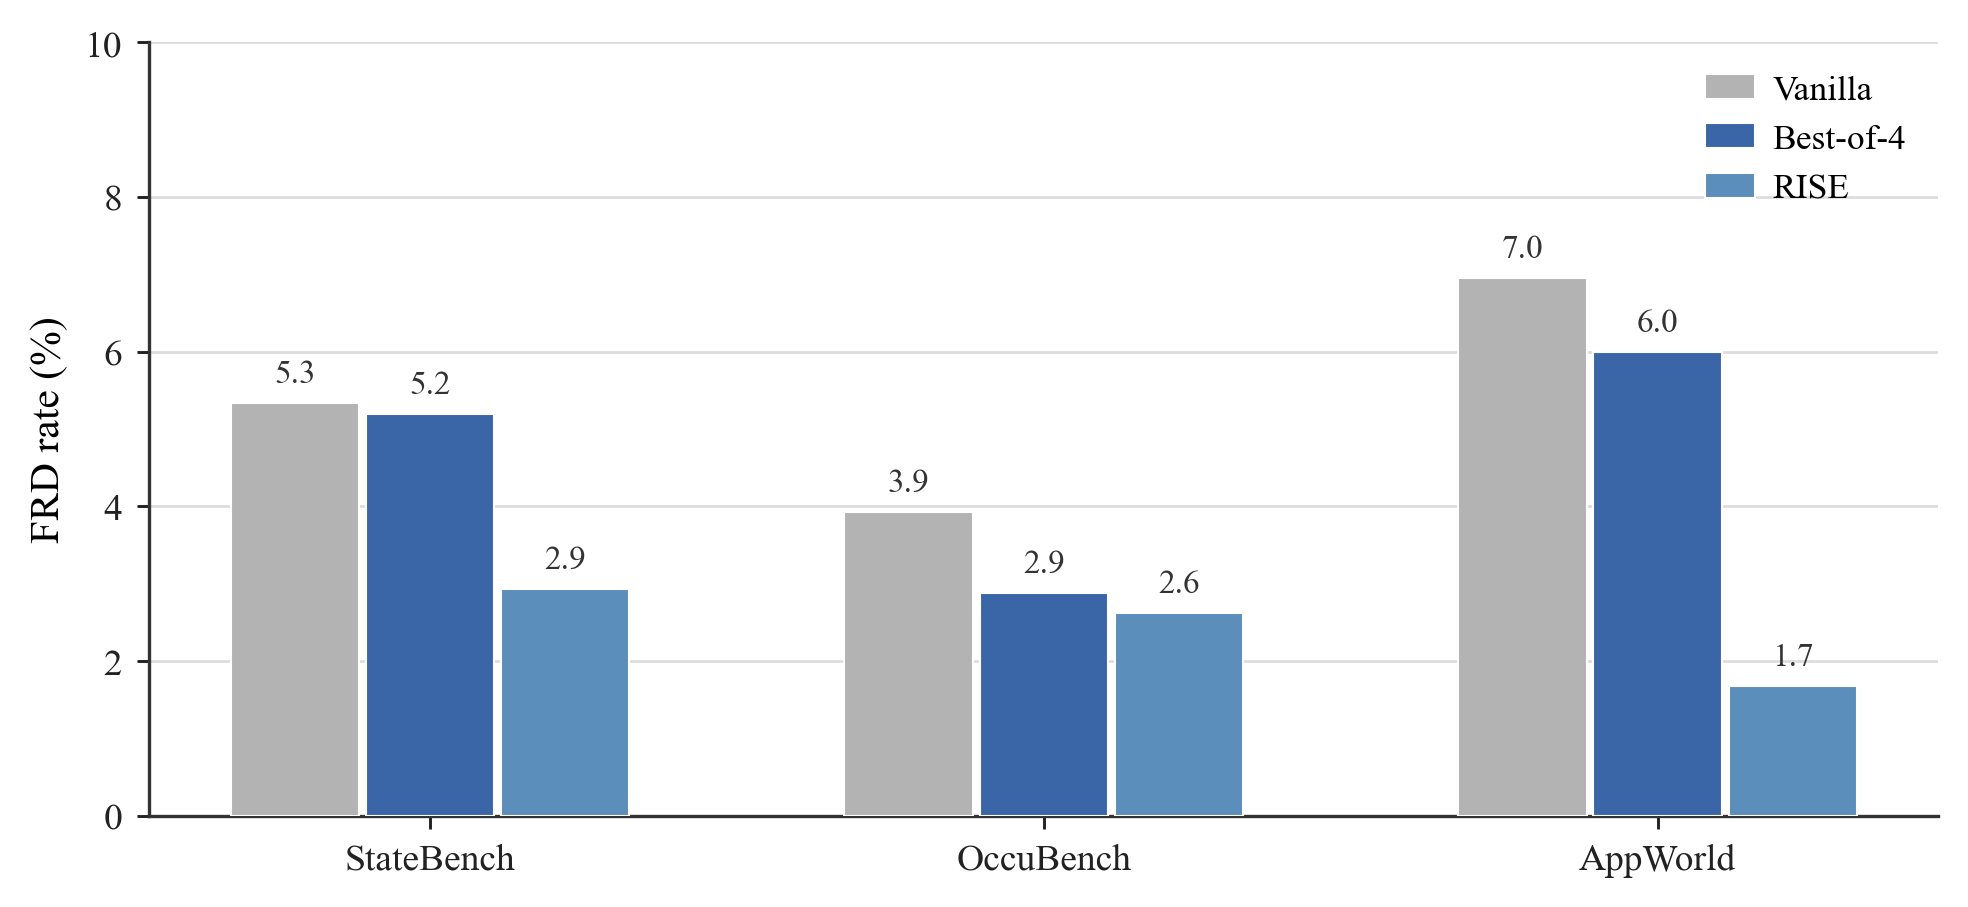
\includegraphics[width=\linewidth]{figures/rise_frd_prevalence.png}
\par\vspace{4pt}\raggedright\normalfont\normalsize
(a) FRD prevalence.\par
\end{minipage}\hspace{0.02\linewidth}
\begin{minipage}[t]{0.46\linewidth}
\vspace{0pt}
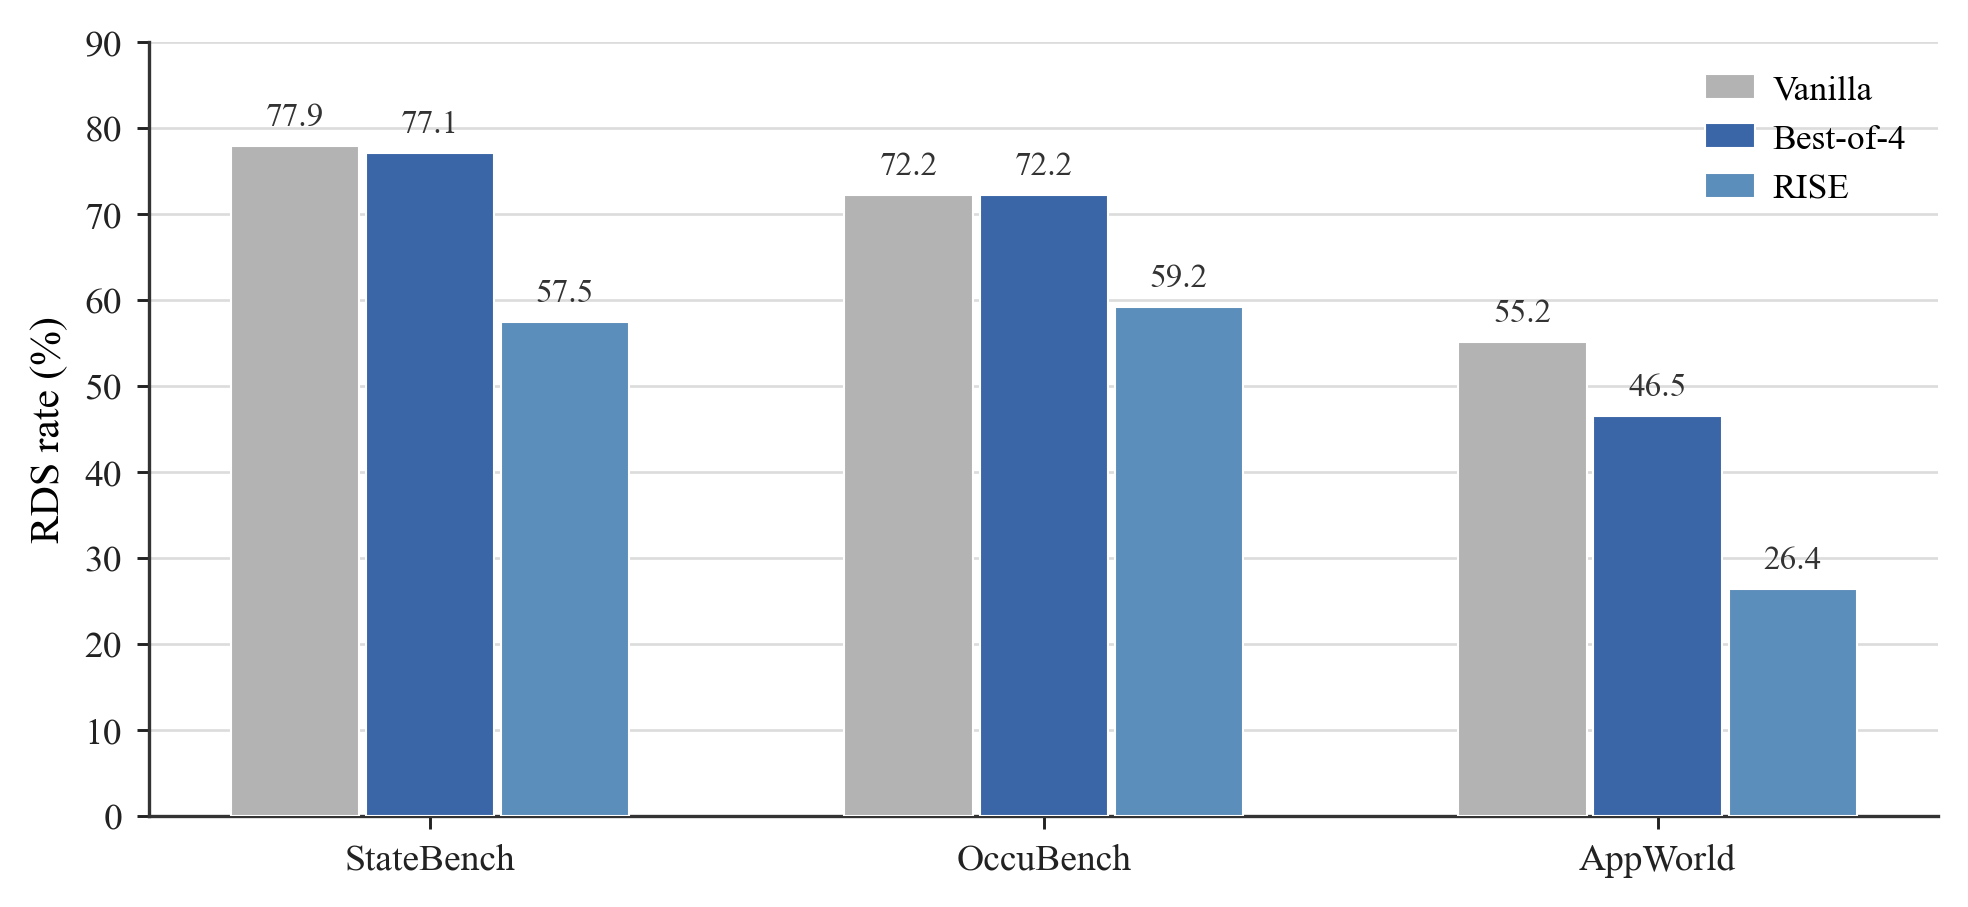
\includegraphics[width=\linewidth]{figures/rise_rds_prevalence.png}
\par\vspace{4pt}\raggedright\normalfont\normalsize
(b) RDS prevalence.\par
\end{minipage}
\caption{DeepSeek-v4.1-Flash: detected FRD (a) and public RDS evidence (b) in final selected trajectories on StateBench, OccuBench, and AppWorld. Values are task-level descriptive measurements under the stated protocol.}
\label{fig:analysis-frd-rds}
\end{figure}

\subsection{Matched risk-positive cohorts}
Finally, we compare completion on fixed task cohorts selected from independently evaluated baseline trajectories. Vanilla-FRD-positive and Vanilla-RDS-positive comprise tasks whose Vanilla trajectories contain detected FRD and public RDS evidence, respectively; all methods share the same task set and denominator within each cohort. Positive denotes risk observed under the current protocol. Figure~\ref{fig:cohort-success} shows that RISE improves over Vanilla on both cohorts across all three benchmarks. FRD-positive gains are largest on OccuBench and StateBench, at 26.7 and 22.5 percentage points; OccuBench also gains 15.6 points on RDS-positive tasks. However, on the StateBench RDS-positive cohort, RISE trails Best-of-4 by 0.7 points, so improvement over Vanilla does not imply uniform superiority over both baselines.

\begin{figure}[!htb]
\centering
\begin{minipage}[t]{0.46\linewidth}
\vspace{0pt}
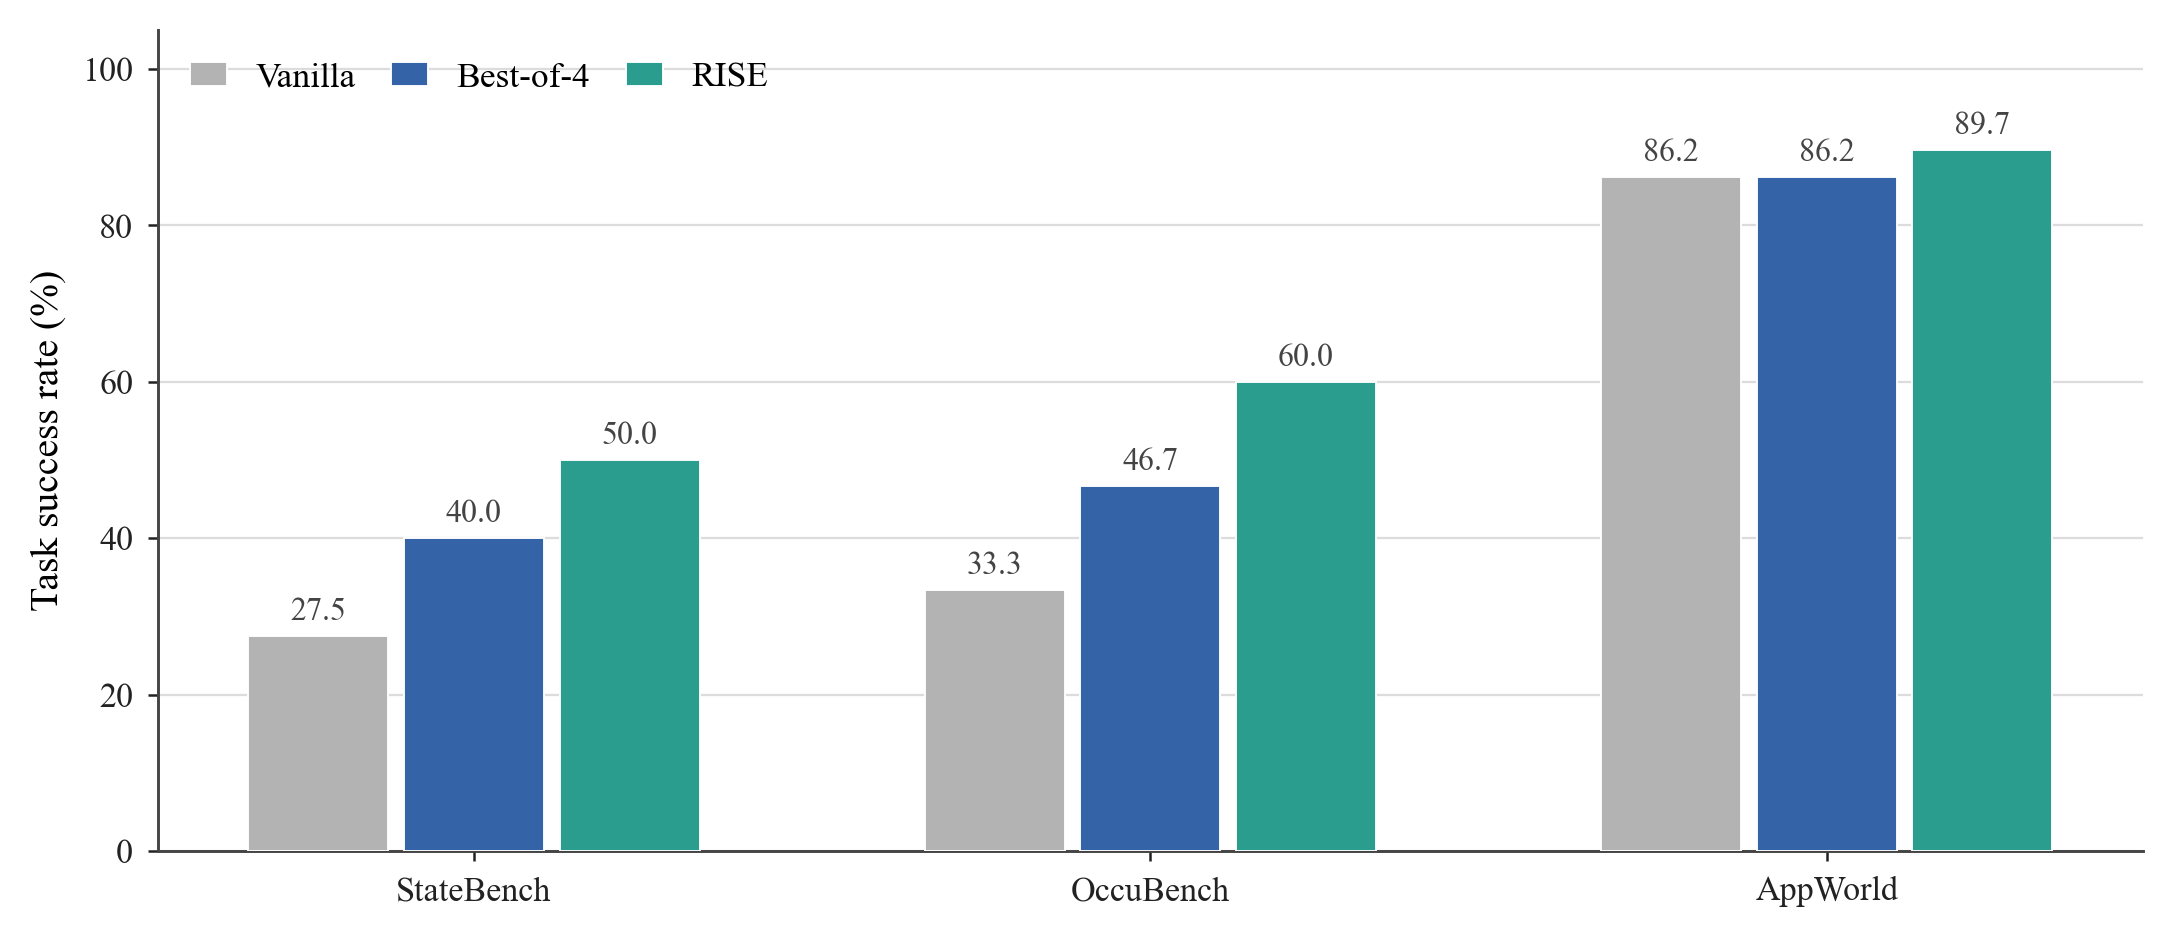
\includegraphics[width=\linewidth]{figures/cohort_frd_success.png}
\par\vspace{4pt}\raggedright\normalfont\normalsize
(a) Vanilla-FRD-positive tasks.\par
\end{minipage}\hspace{0.02\linewidth}
\begin{minipage}[t]{0.46\linewidth}
\vspace{0pt}
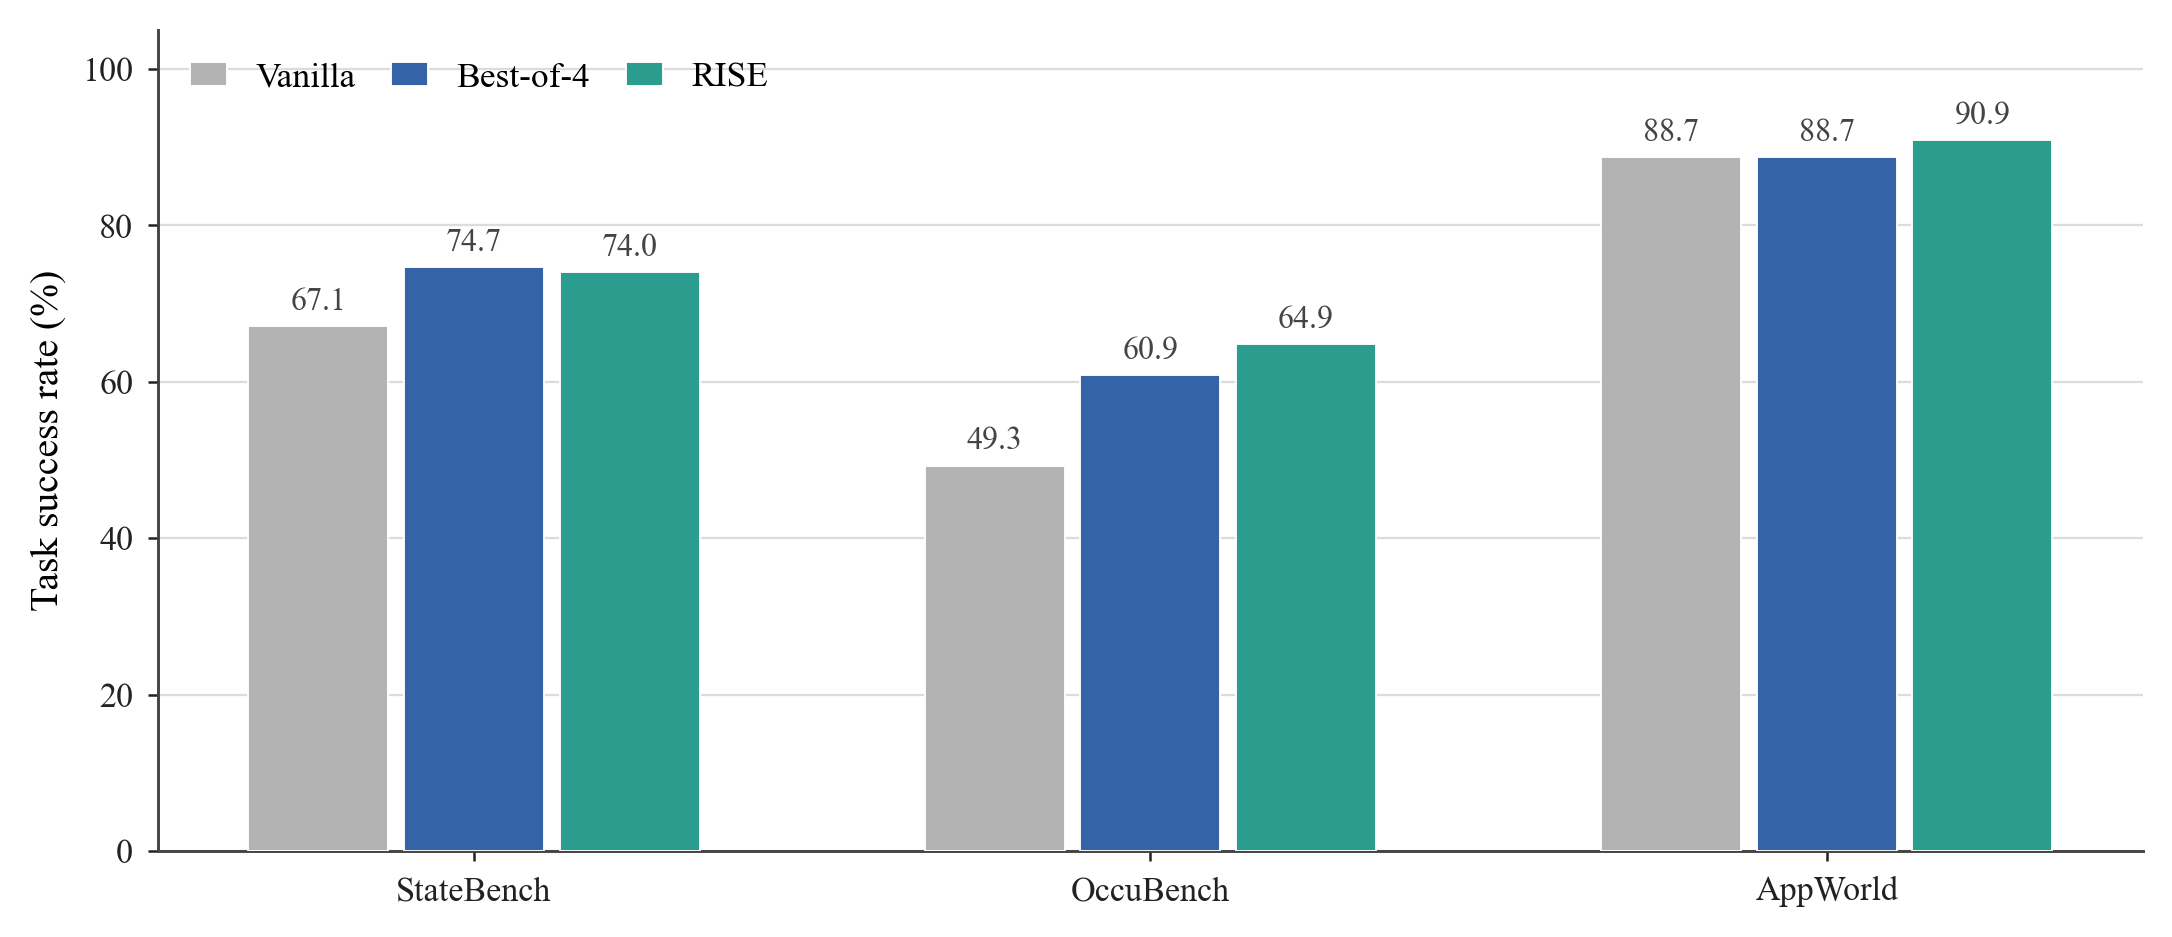
\includegraphics[width=\linewidth]{figures/cohort_rds_success.png}
\par\vspace{4pt}\raggedright\normalfont\normalsize
(b) Vanilla-RDS-positive tasks.\par
\end{minipage}
\caption{DeepSeek-v4.1-Flash task success on fixed Vanilla-positive cohorts across StateBench, OccuBench, and AppWorld. Tasks are selected by Vanilla trajectories containing (a) detected FRD or (b) public RDS evidence; each denominator is identical across methods.}
\label{fig:cohort-success}
\end{figure}

Figure~\ref{fig:best4-cohort-success} applies the same procedure to tasks whose Best-of-4 trajectories contain FRD or RDS evidence, again fixing each cohort across methods. RISE exceeds Vanilla and matches or exceeds Best-of-4 in every reported cohort, including the indicated ties, reaching 92.0\% on AppWorld FRD-positive tasks. Together, these results support improved completion on tasks selected by independently observed baseline risk. RISE starts from its own Vanilla rollout, rather than continuing or repairing the Best-of-4 trajectory used to define the cohort.

\begin{figure}[!htb]
\centering
\begin{minipage}[t]{0.46\linewidth}
\vspace{0pt}
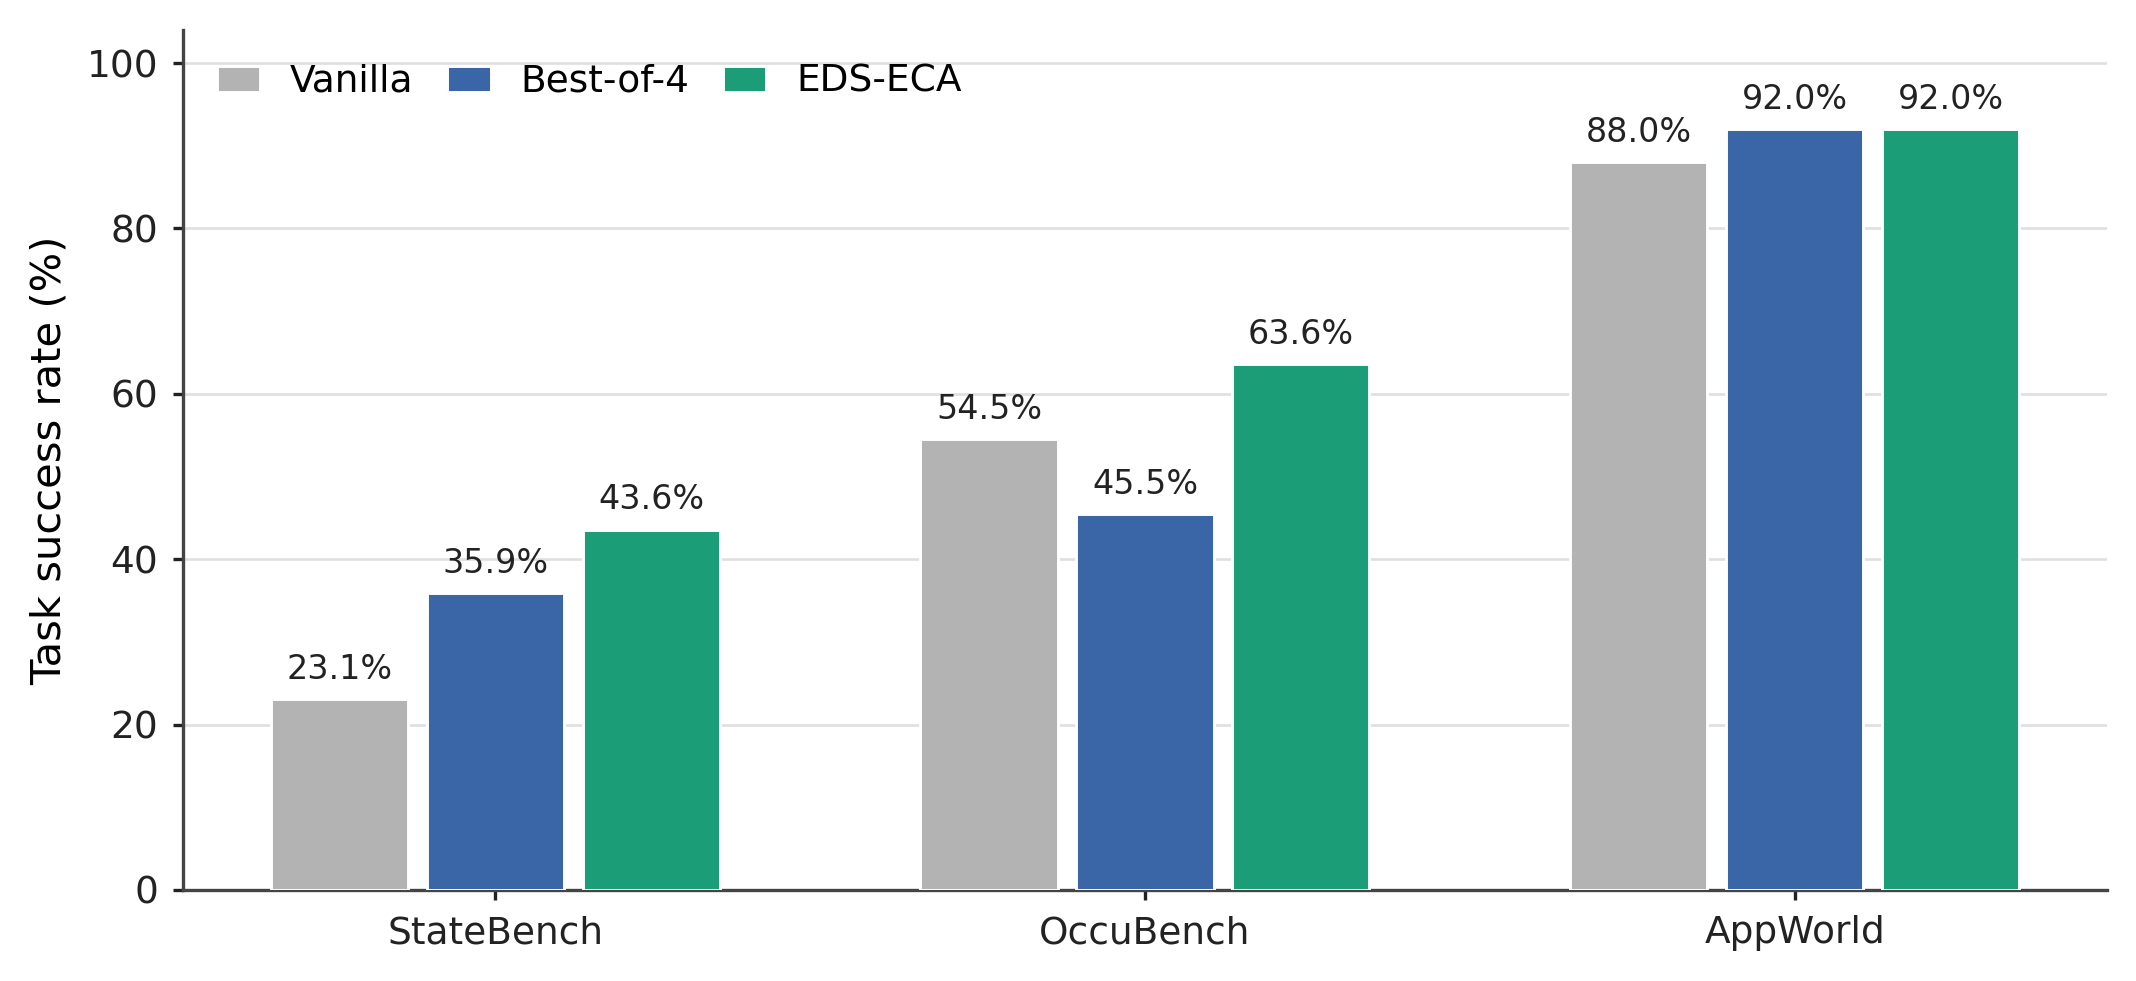
\includegraphics[width=\linewidth]{figures/best4_frd_success.png}
\par\vspace{4pt}\raggedright\normalfont\normalsize
(a) Best-of-4-FRD-positive tasks.\par
\end{minipage}\hspace{0.02\linewidth}
\begin{minipage}[t]{0.46\linewidth}
\vspace{0pt}
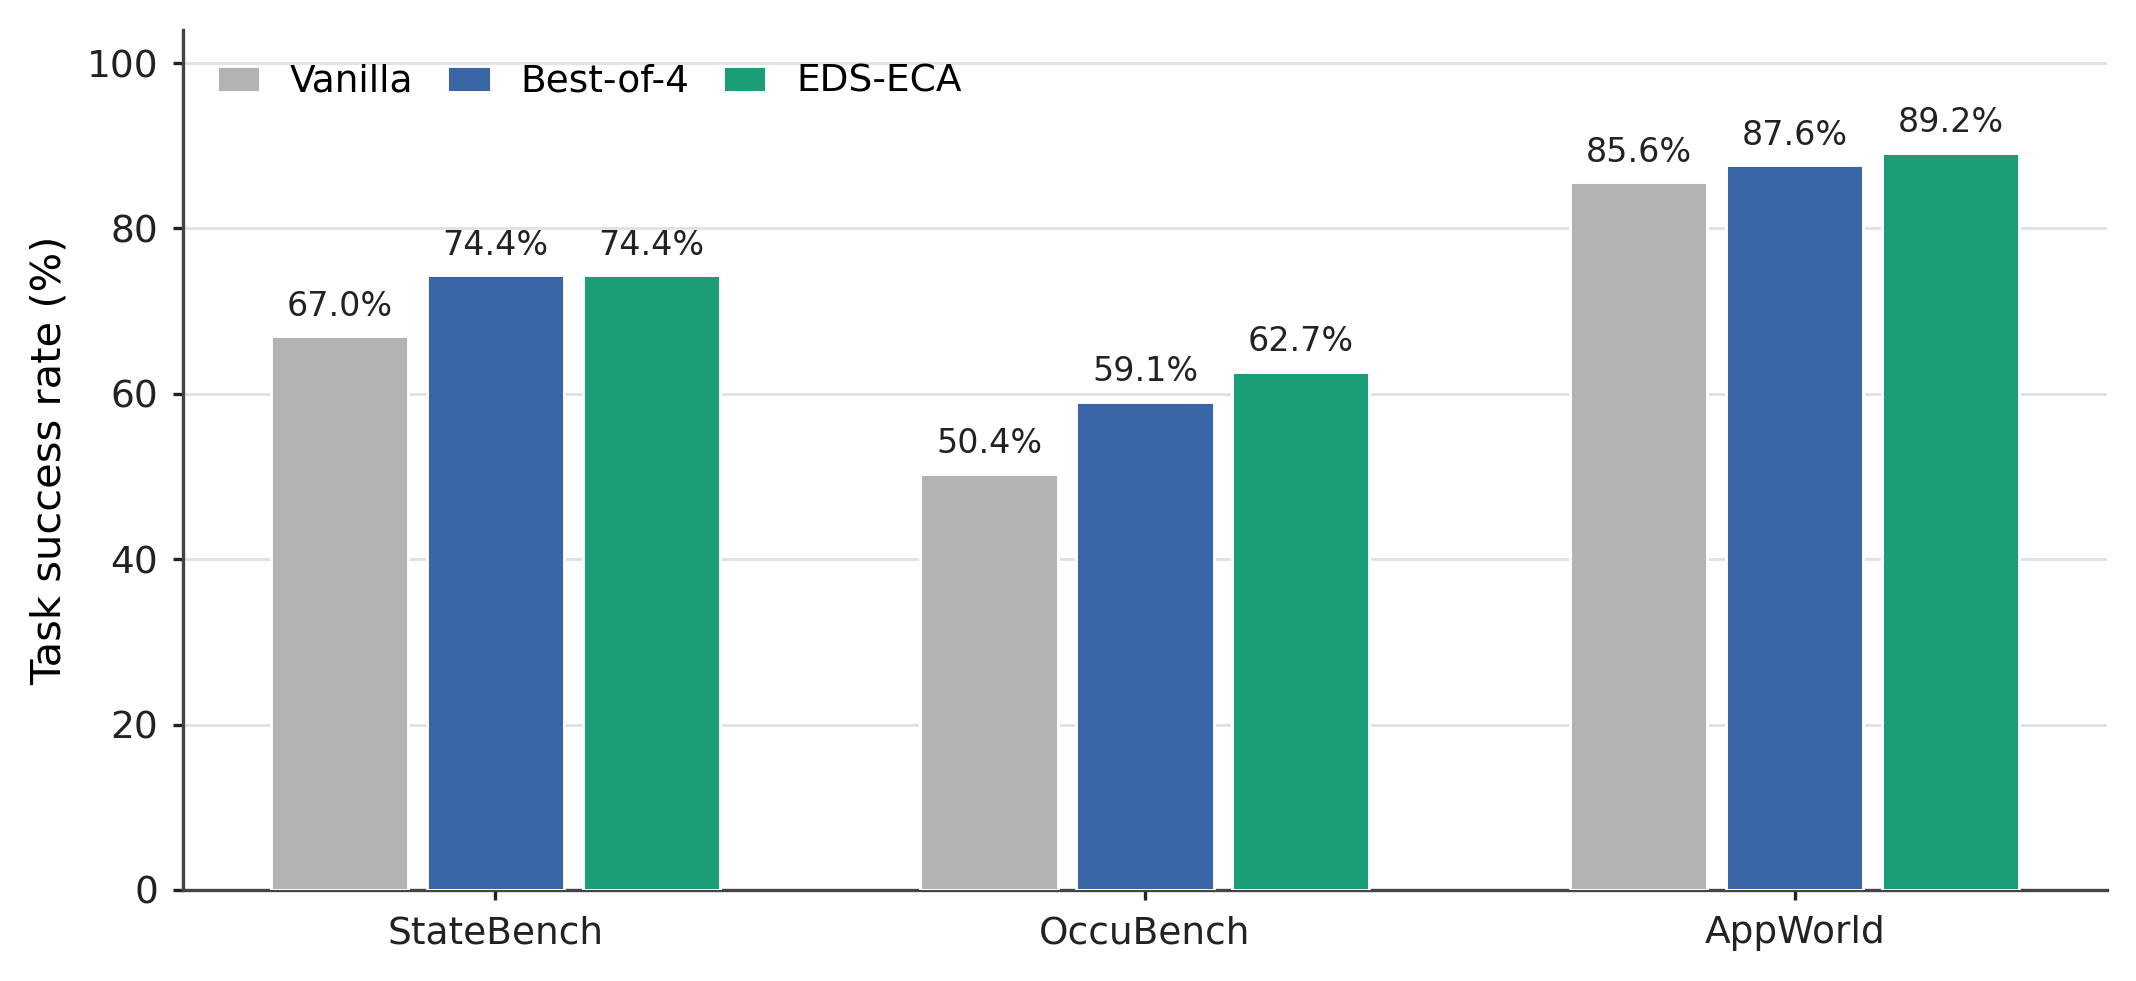
\includegraphics[width=\linewidth]{figures/best4_rds_success.png}
\par\vspace{4pt}\raggedright\normalfont\normalsize
(b) Best-of-4-RDS-positive tasks.\par
\end{minipage}
\caption{DeepSeek-v4.1-Flash task success on fixed Best-of-4-positive cohorts across StateBench, OccuBench, and AppWorld. Tasks are selected by Best-of-4 trajectories containing (a) detected FRD or (b) public RDS evidence; each denominator is identical across methods.}
\label{fig:best4-cohort-success}
\end{figure}

\FloatBarrier
\section{Related Work}
Prior work establishes the test-time selection and tool-calling context for RISE's public-event recovery loop.

\paragraph{Tool-calling systems and empirical design.} OAgents studies design choices in tool-using LLM systems and emphasizes reproducible comparisons across configurations \citep{oagents2025}. Its companion test-time-compute study evaluates parallel sampling, sequential revision, verification, and result merging; the released four-rollout setting uses Best-of-$N$ with list-wise verification and result merging \citep{oppo_tts2025}. Our Best-of-4 comparisons follow the respective OAgents configuration on all four benchmarks. RISE addresses the complementary question of how public recovery evidence and bilateral event credit can guide later complete rollouts while preserving an accepted trajectory.

\paragraph{Tool calling and trajectory representations.} ReAct established the interleaving of LLM reasoning, tool calls, and observations \citep{yao2023react}. Other work improves controller training through verified tool-use data and tutorial-guided trajectory synthesis, while world-model methods represent action-conditioned state transitions before action selection \citep{mat2025,agenttrek2025,wma2025}. These approaches improve tool-use capability or observation representation. RISE instead targets the recovery boundary after an unexpected result by converting public traces into events, identifying RDS evidence, and using provenance to determine what a later rollout may reuse.

\paragraph{Test-time scaling and iterative selection.} Self-consistency samples multiple reasoning paths, Tree of Thoughts expands and evaluates intermediate states, and Reflexion feeds verbal feedback into later attempts \citep{wang2023selfconsistency,yao2023tree,shinn2023reflexion}. Layered proposal-and-aggregation methods likewise frame scaling as repeated proposal and aggregation across stages \citep{moa2024}. RISE shares the premise that additional inference can improve a fixed model, but its scaling unit is an accepted tool-calling trajectory with a public event view. Material disagreement yields both a whole-trajectory decision and bilateral event guidance, so even a rejected proposal can influence the next fresh rollout.

\section{Conclusion}

RISE uses public recovery evidence to guide test-time scaling for LLM tool calling. Within one accepted-incumbent search, RDS focuses the next fresh execution, complete-candidate comparison determines which trajectory is retained, and source-constrained bilateral event feedback determines which structures are carried into later rounds. Across four benchmarks, the three evaluated LLMs improve over Vanilla and Best-of-4 on aggregate metrics; the ablations support the roles of explicit recovery focus and cross-round feedback. Recovery analyses are descriptive under their stated adjudication coverage. RISE depends on informative public traces and a reliable candidate comparator, its event credit is structural guidance rather than correctness certification, and its current execution setting requires fresh task environments.

\FloatBarrier
\subsection*{AI Use Statement}
Generative AI tools assisted with early research organization, code documentation, and language drafting. The paper reports the aggregate tables and analyses supplied for this revision; the authors are responsible for the final claims, source data, and released code.

\subsection*{Reproducibility Statement}
Reproducibility materials include the RISE core, benchmark adapters, selector prompts, event schemas, test configurations, and evaluation scripts. The supplementary material records task manifests, seeds, model endpoints, selector budgets, verifier settings, and per-task paired outputs. Online components exclude evaluator outcomes, reward, hidden state, and gold action sequences.

\bibliography{references}
\bibliographystyle{iclr2027_conference}

\appendix
\section{Implementation Details}
\label{app:implementation}
The public event adapter supplies benchmark-specific parsing to the single RISE loop. StateBench exposes tool calls, arguments, and results, and builds atomic events, transaction groups, recovery windows, and recovery decisions. OccuBench maps action-observation traces into a compatible representation. AppWorld uses persistent Python/API interactions, explicit exceptions, and API result shapes, without requiring the full recovery hierarchy. Normal business rejection alone does not establish an execution anomaly. The pseudocode names benchmark-specific transitions explicitly: no-disagreement retains the incumbent and does not invoke selection; fallback retains the incumbent without creating comparison credit; and runner errors follow the configured exit or resume policy. No branch creates event credit without a valid selected/rejected comparison.

\paragraph{Algorithmic summary.} The formal pseudocode is placed here so that the main method section can focus on the RISE mechanism and its evidence flow. The schedule may contain any configured number of proposal rounds; the A/B/C/D labels used in the case study are only an ordering convention.

\begin{algorithm}[H]
\caption{RISE: Recovery-Informed Scaling via Events}
\label{alg:rise}
\small
\begin{algorithmic}[1]
\Require Task $x$, benchmark interface $b$, proposal schedule $\mathcal{S}$
\State $I\gets\operatorname{VanillaFreshRollout}_b(x)$; $C\gets\varnothing$; initialize $H$
\For{stage $s\in\mathcal{S}$}
  \State $V_I\gets A_b(I)$; $\mathcal{F}\gets f_b(V_I,C,H)$
  \State $P\gets\operatorname{FreshRollout}_{b,\theta}(x,\mathcal{F},s)$; $V_P\gets A_b(P)$
  \State $D\gets d_b(V_I,V_P)$
  \If{$D=0$}
    \State $(I,C,H)\gets\operatorname{NoDisagreementUpdate}_b(I,C,H)$
    \State \textbf{continue}
  \EndIf
  \State $q\gets\operatorname{Select}_b(x,V_I,V_P)$ with runner error/resume handling
  \If{$q$ is a returned fallback}
    \State $(I,C,H)\gets\operatorname{FallbackUpdate}_b(I,C,H,q)$
    \State \textbf{continue}
  \EndIf
  \State $(V^s,V^r)\gets\operatorname{SelectedRejected}(V_I,V_P,q)$
  \State $C\gets u_b(V^s,V^r,D,q,C)$
  \If{$q=\mathrm{prop}$} \State $I\gets P$ \EndIf
  \State $H\gets\operatorname{HistoryUpdate}_b(H,D,q)$
\EndFor
\State \Return $I$
\end{algorithmic}
\end{algorithm}

\paragraph{StateBench event credit.}
Let $E_s$ and $E_r$ be the selected and rejected event sets and $\mathcal{B}=\{\api{REJECTED},\api{FAILED},\api{ERROR}\}$. Before deterministic sorting and truncation, preserve eligibility is
\begin{equation}
\begin{split}
\mathcal{P}(E_s,E_r)=\{e\in E_s:\;&\operatorname{result}(e)\notin\mathcal{B}\ \land\\
&[\operatorname{shape}(e)\notin\operatorname{Shape}(E_r)\ \lor\\
&\operatorname{class}(e)\in\{\mathrm{mutation},\mathrm{verification}\}]\}.
\end{split}
\label{eq:preserve}
\end{equation}
Here, $\operatorname{Shape}(E_r)$ is the set of rejected-side event shapes. A shape includes operation, event class, tool, entity-field names, argument keys, result class, and interaction type; it excludes literal argument values. The implementation sorts eligible events and retains at most six. If the set is empty, it falls back to the last three selected-side events whose results lie outside $\mathcal{B}$. This includes \api{UNKNOWN}, so eligibility does not certify verified success.

Avoid eligibility uses rejected-side risk identifiers, failure results, structural differences, and mutation/verification rules; sorting retains at most six events. The current transaction groups cover all atomic events. Avoid membership therefore identifies structures for further scrutiny without pinpointing a local error. OccuBench and AppWorld instead validate model-nominated preserve/avoid identifiers against the selected/rejected event sets before structural projection. Their no-disagreement, fallback, and history updates follow their existing runners.

\paragraph{Illustrative bilateral dependency.}
Let the selected event set be $E_s=\{e_o,e_v\}$, with both results outside $\mathcal{B}$. Event $e_o$ is neither mutation nor verification, and $e_v$ is verification. Assume both comparisons have material disagreement and retain this trajectory. If rejected candidate $R_1$ contains $\operatorname{shape}(e_o)$, preserve contains only $e_v$; if $R_2$ lacks that shape, preserve contains both events. Equation~\ref{eq:preserve} yields this conditional example; it is not an experimental observation. The example isolates how a rejected candidate changes guidance without changing the incumbent.

\subsection{Verified case-study trace}
\label{app:case-study}
The two case-study figures use AppWorld Test-Challenge task \api{7264edc\_2}. The following record preserves the verified stage boundaries while omitting non-executable intermediate messages.
\begin{table}[!htb]
\centering
\scriptsize
\caption{Verified stages for the AppWorld case study.}
\label{tab:case-study-trace}
\begin{tabular}{p{0.17\linewidth}p{0.75\linewidth}}
\toprule
Trace & Verified events \\
\midrule
Baseline A & A01--A07 planning; A08 \api{show\_drafts()} without \api{access\_token} returns 401; A28--A36 obtains credentials and logs in; A50 repeats the read without the token and fails again. \\
Candidate D & D01--D04 explores, logs in, and reads documentation; D05--D10 still include failed unauthenticated reads; D11 inspects the \api{show\_drafts} specification; D12 supplies \api{access\_token}; D14--D20 process drafts and inspect remaining state; D21 completes the task and the official evaluation passes 4/4 checks. \\
Selection & PLV(A,B) retains A; PLV(A,C) retains A; PLV(A,D) selects D. Each candidate runs in a fresh environment, and D receives a public frontier targeting A50 plus a generic \api{FAILURE\_RECOVERY} instruction. \\
\bottomrule
\end{tabular}
\end{table}

\section{Claim-Evidence Audit}
\label{app:evidence}
The main results report StateBench, AppWorld, OccuBench, and DeepPlanning Travel under the common name RISE. StateTrace-DSR, StateTrace-EDS-ECA, StateBench-EDS-ECA, and Faithful v3 (EDS-ECA) are implementation names for the supplied RISE results. Best-of-4 uses the respective OAgents comparison configuration. The main tables identify each model, language, and evaluation cohort.

AppWorld Test-Normal and Test-Challenge contain 168/417 tasks and 56/139 scenario groups, respectively; differences use unrounded counts. StateBench retains the supplied precision for PASS@1, PASS$^5$, and UX, with differences computed from reported scores. OccuBench PASS@1 and differences use success counts over 382 instances. DeepPlanning Delivery differences use counts where available; other differences use reported scores. The prevalence and matched-cohort figures in Sections 2 and 5 retain the original DeepSeek-v4.1-Flash analyses on the three tool-calling benchmarks; they do not extend recovery analysis to the additional models, AppWorld Test-Normal, or DeepPlanning.

\end{document}
